\documentclass{nku}
\usepackage{ctex} % 使用ctex包以支持中文
\usepackage[fontset=none]{ctex} % 不使用ctex的默认字体设置
\usepackage{xeCJK} % 加载xeCJK宏包处理中文  
\setCJKmainfont[AutoFakeBold]{FangSong} % 启用伪粗体
% 自定义加粗命令,使用仿宋字体并启用伪粗体
\newCJKfontfamily{\jiacu}[AutoFakeBold = {3.17}]{FangSong}
\usepackage{subfigure}
\usepackage{listings}
\usepackage{amsmath}
\usepackage{algorithm}
\usepackage{algorithmic}
\usepackage{xcolor}  % 如果需要自定义颜色
\lstset{
    basicstyle=\ttfamily\footnotesize,  % 等宽字体和小字体
    keywordstyle=\color{blue!70}\bfseries,  % 关键词为蓝色加粗
    stringstyle=\color{orange},    % 字符串为橙色
    commentstyle=\color{green!50!black}\itshape, % 注释为绿色斜体
    showstringspaces=false,  % 不显示空格
    numbers=left,  % 在左边显示行号
    numberstyle=\tiny\color{gray},  % 行号为小号灰色字体
    frame=lines,  % 仅在代码上下方添加线条
    rulecolor=\color{gray},  % 边框颜色
    breaklines=true,  % 自动换行
    breakatwhitespace=true,  % 在空格处换行
    backgroundcolor=\color{gray!10},  % 背景色为浅灰色
    tabsize=4,  % Tab 键的宽度
    captionpos=b,  % 标题在下方
    aboveskip=1em,  % 上方留有间距
    belowskip=1em,  % 下方留有间距
    morekeywords={self},  % 额外高亮关键词
}

% =============================================
% Part 0 Edit the info
% =============================================

\major{软件工程}
\name{谢国欢}
\title{OpenMP 编程练习}
\stuid{2212906}
\college{软件学院}
\date{\today}
\lab{泰达五区105}
\course{《并行与分布式程序设计》}
\instructor{孙永谦}
\expname{第4次作业}

% 插入代码示例\lstinputlisting[language=MATLAB]{code/do.m}

%插入图片示例
%\begin{figure}[H]
% \centering
% 
\includegraphics[width=0.5\textwidth]{figures/cover.jpg}
% \end{figure}

\begin{document}
\makecover
\tableofcontents
\newpage
\makeheader

\section{梯形积分法的Pthread、OpenMP实现}
\subsection{实验目的}
分别实现课件中的梯形积分法的Pthread、OpenMP版本,熟悉并掌握OpenMP编程方法,探讨两种编程方式的异同。

\subsection{实验要求}
\begin{enumerate}
    \item 问题描述
    \item 算法设计和实现
    \item 实验及结果分析
\end{enumerate}

\subsection{问题描述}
在科学计算和工程应用中,数值积分方法广泛用于解决无法解析求解的积分问题。梯形积分法作为一种常见的数值积分方法,其计算效率和精度使其成为数值积分中基础且重要的算法之一。随着多核处理器和并行计算技术的不断发展,如何提高梯形积分法的计算效率,尤其是在大规模数据处理中的应用,成为了研究的重点。为了提高梯形积分法的性能,使用并行计算技术可以显著加速计算过程。

在多核计算环境下,Pthread和OpenMP是两种常用的并行编程技术。Pthread是较底层的线程库,提供了细粒度的线程控制,而OpenMP则是更高层次的并行编程模型,能够通过简单的指令来实现并行计算。这两种编程模型在性能、可扩展性、编程复杂度等方面存在显著的差异。

本实验旨在将梯形积分法的计算过程分别使用Pthread和OpenMP进行并行化实现,重点探讨两者在性能优化方面的异同。通过对比不同编程方式在处理相同问题时的效率表现,分析各自的优势和局限性。

\textbf{任务目标:}
\begin{enumerate}
    \item 如何使用Pthread实现梯形积分法的并行化
    \item 如何使用OpenMP实现相同的并行化
    \item 探讨在实现过程中,Pthread和OpenMP的编程模型和性能特点有何异同
\end{enumerate}

\subsection{实验设计}
\subsubsection{实验环境}
\begin{itemize}
    \item \textbf{CPU:}Intel Core i7 12700H
    \item \textbf{操作系统:}Windows
    \item \textbf{编译器:}TDM-GCC 10.3.0
    \item \textbf{IDE:}Code::Blocks 20.03
\end{itemize}

\subsubsection{实验数据及方法设置}
\begin{itemize}
    \item 测试函数为$y=x^2$,如下代码所示,测试区间为$0\sim$1,区间分为1000000块:
\begin{lstlisting}[language=C]
double f(double x) {
    // 被积函数
    return x * x;
}
\end{lstlisting}
    \item 两种方式实现的梯形积分法各测试10000次,最后取平均值
    \item 使用 Windows 高精度计时器 QueryPerformance 系列 API 测量执行用时
\end{itemize}


\subsection{实验流程与结果分析}
\subsubsection{基于Pthread的多线程梯形积分法实现}
首先引入相关库,并定义本实验中线程所需结构体。另外,定义一些宏变量,如重复测试次数,线程数(这里我们选择将线程数设定为4,与下述OpenMP版本的线程数一致)
\begin{lstlisting}[language=C]
#include <iostream>
#include <cmath>
#include <windows.h>
#include <pthread.h>
#include <iomanip>

using namespace std;

#define NUM_THREADS 4
#define REPEAT_TIME 10000

struct ThreadData {
    double a, b, h;
    int n, thread_id, num_threads;
    double result;
};
\end{lstlisting}

随后进行针对单个线程的梯形积分法的函数编写,这里实现较为简单,只需按照线程ID进行静态任务分配(考虑到本任务较为均衡,故只使用静态任务),随后再进行梯形积分求解即可。代码如下:
\begin{lstlisting}[language=C]
void* trapezoidal_integration_thread(void* arg) {
    ThreadData* data = (ThreadData*) arg;
    double a = data->a;
    double b = data->b;
    double h = data->h;
    int n = data->n;
    int thread_id = data->thread_id;
    int num_threads = data->num_threads;

    // 计算线程的积分区间
    int local_n = n / num_threads;
    int start = thread_id * local_n + 1;
    int end = (thread_id == num_threads - 1) ? n : start + local_n;

    // 计算部分积分结果
    double local_result = 0;
    for (int i = start; i < end; i++) {
        local_result += f(a + i * h);
    }

    // 返回结果
    data->result = local_result;

    return NULL;
}
\end{lstlisting}

接着进行梯形积分法多线程创建、管理及销毁代码的编写。这里实现逻辑即为先创建多线程分别求解各自的积分,最后将所有线程计算的结果相加。最后依次销毁各线程即可。代码如下:
\begin{lstlisting}[language=C]
double trapezoidal_integration_pthread(double a, double b, int n, int num_threads) {
    double h = (b - a) / n;
    double result = (f(a) + f(b)) / 2;

    pthread_t* threads = new pthread_t[num_threads];
    ThreadData* thread_data = new ThreadData[num_threads];

    // 启动多线程
    for (int i = 0; i < num_threads; i++) {
        thread_data[i].a = a;
        thread_data[i].b = b;
        thread_data[i].h = h;
        thread_data[i].n = n;
        thread_data[i].thread_id = i;
        thread_data[i].num_threads = num_threads;

        pthread_create(&threads[i], NULL, trapezoidal_integration_thread, (void*)&thread_data[i]);
    }

    // 等待所有线程完成
    for (int i = 0; i < num_threads; i++) {
        pthread_join(threads[i], NULL);
        result += thread_data[i].result;
    }

    delete[] threads;
    delete[] thread_data;

    return h * result;
}
\end{lstlisting}

至此,基于Pthread的多线程梯形积分法相关函数编写完毕。
\subsubsection{基于OpenMP的多线程梯形积分法实现}
首先引入OpenMP相关库。在这里,由于在上一步中已经完成了本实验所需变量的定义和辅助库导入,故这里只需导入\textbf{omp}库即可,代码如下:
\begin{lstlisting}[language=C]
#include <omp.h>
\end{lstlisting}

随后进行基于OpenMP的多线程梯形积分法的函数编写,由于不存在数值依赖,故这里只需对求解时累加部分进行并行化即可。具体代码如下:
\begin{lstlisting}[language=C]
double trapezoidal_integration(double a, double b, int n) {
    double h = (b - a) / n;
    double result = (f(a) + f(b))/2;

    #pragma omp parallel for reduction(+:result) num_threads(NUM_THREADS)
    for (int i = 1; i < n; i++) {
        result += f(a + i * h);
    }

    return h * result;
}
\end{lstlisting}

\subsubsection{实验结果及分析}
编写完上述两个版本的代码后,在主函数中进行使用并测试即可,相关主函数测试代码如下:
\begin{lstlisting}[language=C]
int main() {
    double a = 0, b = 1;
    int n = 1000000;
    double area,duration;

    // QueryPerformanceFrequency 和 QueryPerformanceCounter 用于高精度计时
    LARGE_INTEGER frequency, start_time, end_time;
    QueryPerformanceFrequency(&frequency);  // 获取计时器频率
    QueryPerformanceCounter(&start_time);   // 获取开始时间

    for(int i=0;i<REPEAT_TIME;i++)
        area = trapezoidal_integration(a, b, n);

    QueryPerformanceCounter(&end_time);     // 获取结束时间
    duration = (double)(end_time.QuadPart - start_time.QuadPart) / frequency.QuadPart;

    cout<<"OpenMP"<<endl;
    cout << fixed << setprecision(12);
    cout << "Area: " << area << endl;
    cout << "Avg Computation time: " << duration/REPEAT_TIME << " seconds" << endl;

    QueryPerformanceFrequency(&frequency);  // 获取计时器频率
    QueryPerformanceCounter(&start_time);   // 获取开始时间

    for(int i=0;i<REPEAT_TIME;i++)
        area = trapezoidal_integration_pthread(a, b, n, NUM_THREADS);

    QueryPerformanceCounter(&end_time);     // 获取结束时间
    duration = (double)(end_time.QuadPart - start_time.QuadPart) / frequency.QuadPart;

    cout<<"Pthread"<<endl;
    cout << "Area: " << area << endl;
    cout << "Avg Computation time: " << duration/REPEAT_TIME << " seconds" << endl;

    return 0;
}
\end{lstlisting}

最后得到实验结果如下:
\begin{figure}[H]
\centering
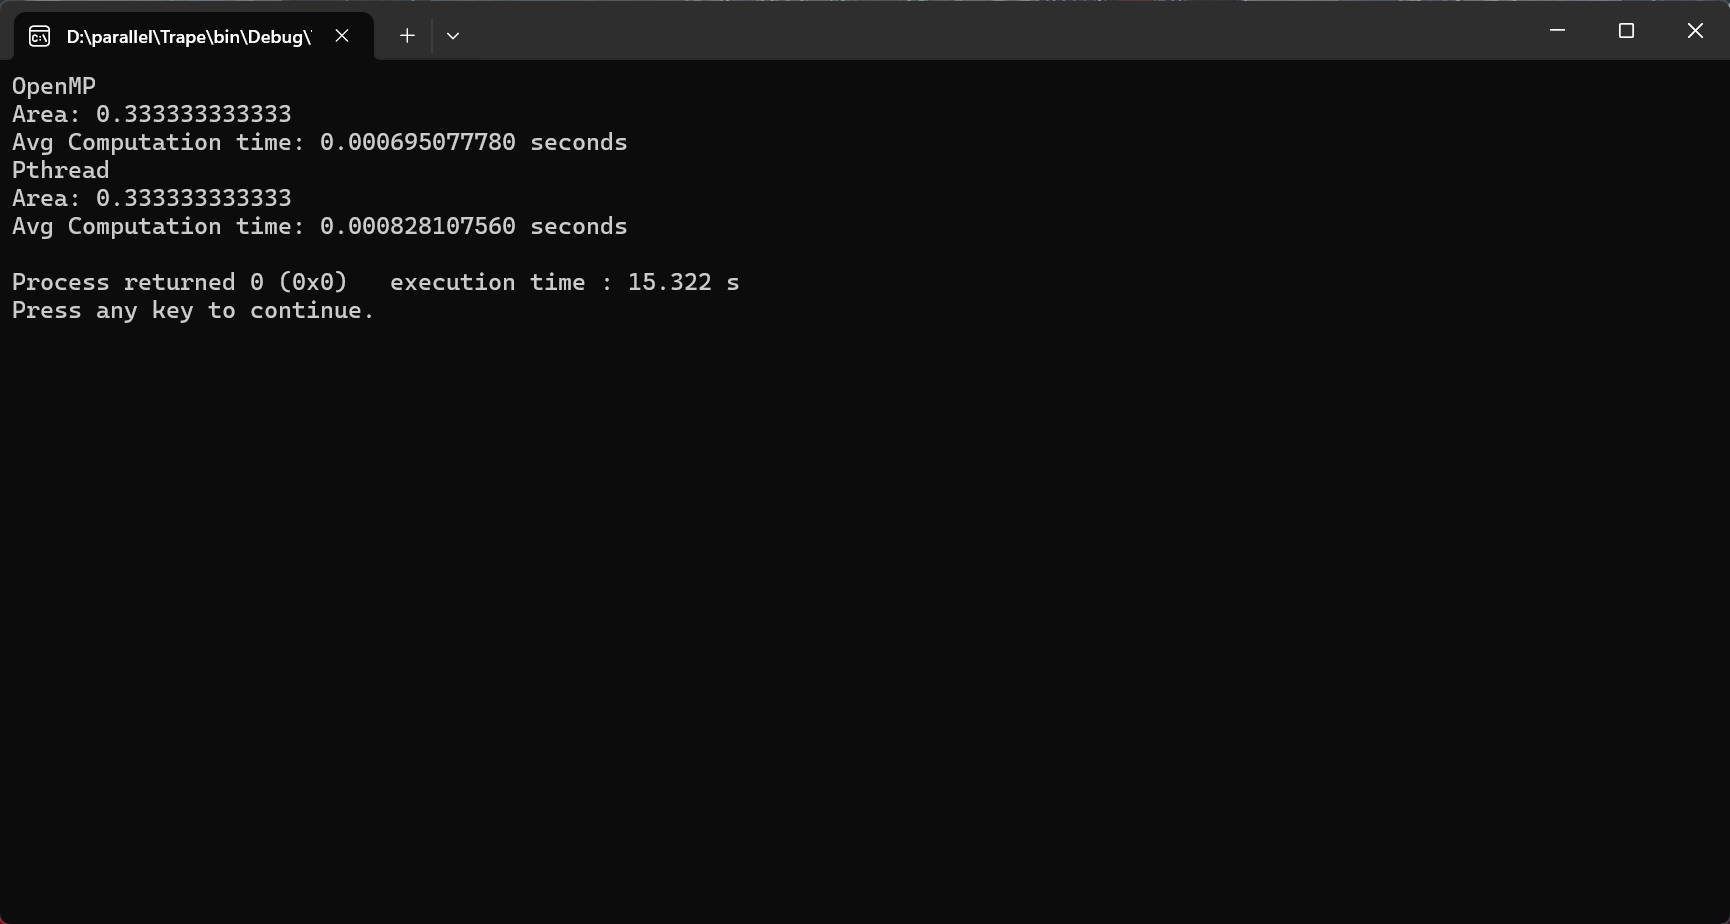
\includegraphics[width=0.8\textwidth]{fig/fig1.jpg}
\end{figure}

可以看到,上述两种方式实现的梯形积分法运行结果良好。即对函数$y=x^2$的区间[0,1]进行积分,最后所得结果为$\frac{1}{3}$。但不同方式实现的梯形积分法的平均运行时间略有差异(基于Pthread实现的方法运行时间略长于基于OpenMP实现的方法运行时间),具体运行时间从上图可得:
\begin{itemize}
    \item \textbf{OpenMP: 0.000695077780 s}
    \item \textbf{Pthread: 0.000828107560 s}
\end{itemize}

出现上述现象也很符合预期,原因如下:
\begin{itemize}
    \item OpenMP的编译器(如GCC、Clang等)能够在编译时进行大量优化。例如,它可能会尝试减少线程之间的通信、优化内存访问模式或使用缓存等策略,从而提升性能。
    \item Pthread的编译器优化较少,因为它更依赖于程序员的手动控制,开发者可能无法像OpenMP一样依赖编译器优化来自动提升性能。
    \item OpenMP通常对多核和多线程硬件进行了高度优化,能够更好地利用现代处理器的特性,例如处理器缓存和NUMA(非统一内存访问)架构。
    \item Pthread虽然灵活,但开发者需要针对具体硬件做细致的优化,这往往需要较深入的硬件知识,否则可能无法达到OpenMP那样的高效。
\end{itemize}

\subsection{两种编程方异同的比较}
OpenMP编程和Pthread编程是两种常见的并行编程模型,它们在设计理念、使用方式、性能调优等方面有着显著的异同。以下是详细的比较:

\begin{enumerate}
    \item \textbf{ 编程抽象级别:}
    \begin{itemize}
        \item \textbf{OpenMP:} 
        \begin{itemize}
            \item OpenMP(Open Multi-Processing)是一个高层次的并行编程模型,它通过编译器指令来实现并行化,而无需手动管理线程。使用OpenMP,开发者只需在现有代码中添加一些简单的\#pragma指令(例如\#pragma omp parallel),编译器会自动将代码并行化,并且处理任务调度、线程创建与销毁等低级细节。
            \item 其设计目标是使并行化代码尽可能简洁,易于理解和维护。
        \end{itemize}
        \item \textbf{Pthread:}
        \begin{itemize}
            \item Pthread(POSIX Threads)是一种较低级的并行编程API,提供了线程创建、同步、调度等功能。开发者需要手动管理线程的生命周期(创建、销毁、同步等)。与OpenMP相比,Pthread提供了更高的灵活性,但这也意味着它需要开发者有更高的并行编程知识。
            \item Pthread更适合那些需要精细控制的并行任务,或者开发者需要定制特定行为时使用。
        \end{itemize}
    \end{itemize}
    \item \textbf{ 并行化模型:}
    \begin{itemize}
        \item \textbf{OpenMP:}
        \begin{itemize}
            \item OpenMP采用的是“任务并行”的模型,允许在代码中通过指令指定哪些部分需要并行执行。它自动处理数据的分配和同步,开发者不需要手动管理线程和任务。
            \item OpenMP支持多种并行策略,包括循环并行、任务并行等。它通过指令控制线程数量、工作共享策略和同步机制等。
        \end{itemize}
        \item \textbf{Pthread:}
        \begin{itemize}
            \item Pthread采用的是“线程并行”的模型,开发者需要显式地创建和管理线程。每个线程执行不同的任务,线程之间需要通过同步原语(如互斥量、条件变量、信号量等)来协调工作。
            \item Pthread提供了更多的控制权,例如开发者可以决定线程的分配策略,线程之间的数据共享方式等。
        \end{itemize}
    \end{itemize}
    \item \textbf{易用性与开发复杂度:}
    \begin{itemize}
        \item \textbf{OpenMP:} 
        \begin{itemize}
            \item OpenMP的设计目标之一是简化并行编程,因此它的使用非常简洁。开发者只需要在现有的串行代码中添加并行化指令,无需考虑底层的线程管理和同步。缺点是,尽管OpenMP可以自动处理许多底层细节,但在一些特殊需求下(例如复杂的线程管理、特定硬件优化),可能不如Pthread灵活。
        \end{itemize}
        \item \textbf{Pthread:}
        \begin{itemize}
            \item Pthread要求开发者显式管理线程和同步机制,因此编写和维护Pthread程序的复杂度较高。开发者需要关注线程创建、调度、同步等底层问题,容易出现线程同步错误或资源竞争问题。
        \end{itemize}
    \end{itemize}
    \item \textbf{线程管理和调度:}
    \begin{itemize}
        \item \textbf{OpenMP:}   
        \begin{itemize}
            \item OpenMP的线程管理是自动化的,开发者不需要显式创建和销毁线程。编译器会根据系统的CPU核心数和任务的负载自动决定线程的数量和任务分配策略。
            \item OpenMP还支持静态和动态调度策略(static、dynamic、guided),可以在运行时调整任务分配的方式,以达到负载均衡。
        \end{itemize}
        \item \textbf{Pthread:}
        \begin{itemize}
            \item Pthread要求开发者手动管理线程的创建和销毁。开发者可以通过设置线程的优先级、调度策略等来精细控制线程的执行方式。
            \item Pthread的调度较为底层,依赖于操作系统的调度器。
        \end{itemize}
    \end{itemize}
    \item \textbf{同步机制:}
    \begin{itemize}
        \item \textbf{OpenMP:} 
        \begin{itemize}
            \item OpenMP提供了内置的同步机制,如\#pragma omp critical用于定义临界区,\#pragma omp barrier用于线程同步等。它自动处理大部分并行化过程中涉及的同步问题。
            \item 对于复杂的同步,OpenMP支持用户定义并行结构和线程间通信,但相对来说,用户可控性较低。
        \end{itemize}
        \item \textbf{Pthread:}
        \begin{itemize}
            \item Pthread提供了更细粒度的同步机制,包括互斥量(pthread\_mutex)、条件变量(pthread\_cond)、读写锁(pthread\_rwlock)等。开发者可以根据实际需求灵活选择同步工具,处理线程间的资源共享和竞态条件。
            \item 需要开发者精确控制,若同步不当可能导致死锁、资源竞争等问题。
        \end{itemize}
    \end{itemize}
    \item \textbf{性能与优化:}
    \begin{itemize}
        \item \textbf{OpenMP:}  
        \begin{itemize}
            \item OpenMP的性能优化通常依赖于编译器的优化能力。现代编译器(如GCC、Clang)会自动为并行化代码进行一些优化,例如减少线程之间的同步开销、优化内存访问模式等。但在一些需要精细控制硬件资源或优化并行任务调度的场景下,OpenMP的自动化管理可能不如Pthread灵活。
        \end{itemize}
        \item \textbf{Pthread:}
        \begin{itemize}
            \item Pthread由于其低级的控制能力,通常可以获得更高的性能优化,特别是在需要控制线程调度、内存访问模式或与硬件特性紧密相关的优化时。
            \item 然而,这种灵活性要求开发者具备更高的并行编程技巧(在本次实验中,所实现的基于Pthread的梯形积分法性能就略差于基于OpenMp的梯形积分法性能)
        \end{itemize}
    \end{itemize}
    \item \textbf{跨平台支持与兼容性:}
    \begin{itemize}
        \item \textbf{OpenMP:} 
        \begin{itemize}
            \item OpenMP是跨平台的,广泛支持多种操作系统和硬件架构。它通常依赖于编译器(如GCC、Intel Compiler、Clang等)来提供支持,因此,OpenMP代码能够在支持该标准的编译器上无缝运行。并且其代码易于迁移(具体实现如setenv OMP\_SCHEDULE GUIDED,4 [csh, tcsh]/export OMP\_SCHEDULE=GUIDED,4 [sh, ksh, bash]等)
        \end{itemize}
        \item \textbf{Pthread:}
        \begin{itemize}
            \item Pthread是基于POSIX标准的线程库,支持UNIX-like系统(如Linux、macOS、BSD等)。在Windows平台上,Pthread需要通过第三方库进行支持。
            \item 但其代码迁移难度较大,通常实现同一任务要针对不同操作系统或平台进行分别编程。
        \end{itemize}
    \end{itemize}
\end{enumerate}

具体差异比较如下:
\begin{table}[H]
    \centering
    \caption{OpenMP与Pthread的对比}
    \begin{tabular}{lcc}
    \toprule
    \textbf{特性} & \textbf{OpenMP} & \textbf{Pthread} \\
    \midrule
    抽象级别 & 高层次(编译器指令) & 低层次(API函数) \\
    易用性 & 简单,适合快速并行化现有代码 & 灵活,但需要更复杂的线程管理 \\
    并行模型 & 任务并行,自动调度 & 线程并行,手动调度 \\
    线程管理 & 自动管理(由编译器处理) & 手动管理(由程序员处理) \\
    同步机制 & 自动同步或简单指令 & 手动同步(互斥量、条件变量等) \\
    性能优化 & 编译器优化,适用于常见任务 & 灵活优化,适用于高性能需求 \\
    跨平台支持 & 跨平台,依赖于编译器 & 跨平台,依赖于操作系统 \\
    适用场景 & 任务简单,负载均衡需求较高 & 需要精细控制和优化,复杂的任务 \\
    \bottomrule
    \end{tabular}
    \label{table:OpenMP_vs_Pthread}
\end{table}

因此,在具体任务中选择OpenMP还是Pthread取决于任务的复杂度和对性能的要求:
\begin{itemize}
    \item 如果需要快速并行化代码,且任务较简单,OpenMP是一个更方便的选择。
    \item 如果需要更高的灵活性,并且能够处理线程管理、同步等复杂问题,Pthread可能是更合适的选择。
\end{itemize}

\subsection{思考总结}
在这次实验中,我深入探索了Pthread和OpenMP两种并行编程模型在梯形积分法中的应用。通过实验,我对这两种编程方式的优缺点有了更深刻的理解。

首先,OpenMP的高层次抽象和简洁的编程方式让我感受到其在快速并行化现有代码中的优势。通过简单的编译器指令,我能够轻松实现并行化,并且在性能上也得到了显著提升。这种自动化的线程管理和调度机制,极大地降低了编程复杂度,使得我可以将更多精力放在算法优化上。

另一方面,Pthread提供了更细粒度的控制能力,尽管编程复杂度较高,但它让我对线程的管理和同步有了更深入的理解。在实现过程中,我需要手动处理线程的创建、销毁和同步,这让我意识到在某些需要精细控制的场景下,Pthread的灵活性是无可替代的。

通过对比这两种编程方式,我认识到在选择并行编程模型时,需要根据具体任务的复杂度和性能需求进行权衡。OpenMP适合快速实现并行化,而Pthread则适合需要精细控制的复杂任务。总的来说,这次实验不仅让我掌握了两种并行编程技术,还让我对并行计算的设计理念有了更深刻的感悟。未来,我希望能将这些经验应用到更复杂的并行计算任务中,进一步提升程序的性能和效率。

\section{多个数组排序(OpenMP版)}
\subsection{实验目的}
对于课件中“多个数组排序”的任务不均衡案例进行OpenMP编程实现(规模可自己调整),并探索不同循环调度方案的优劣。提示:可从任务分块的大小、线程数的多少、静态动态多线程结合等方面进行尝试,探索规律。

\subsection{实验要求}
\begin{enumerate}
    \item 问题描述
    \item 算法设计和实现
    \item 实验及结果分析
\end{enumerate}

\subsection{问题描述}
在并行计算中,多个数组排序任务的调度和执行往往受到任务划分、线程分配、以及并行策略选择
等因素的影响。对于大规模数组排序任务,通过合理的任务分块、线程数调整以及静态/动态多线程结
合等方式,能够提高任务执行的效率。然而,由于任务间负载可能存在不均衡的情况,如何有效地划分
任务,避免某些线程负担过重,成为提升性能的关键。
任务目标

\textbf{任务目标:}
\begin{enumerate}
    \item 复现多个数组排序的任务不均衡问题,进行实验和调优,探索影响并行性能的因素。
    \item 任务分块的大小:尝试不同的任务划分策略(这里主要是对动态任务分配时粒度大小进行实验)来研究对性能的影响。
    \item 线程数的选择:探索线程数的增减对性能的影响,评估线程过多或过少的情况。
    \item 考虑动态粒度的动态任务分配以优化负载不均衡的情况。
\end{enumerate}

\subsection{实验设计}
\subsubsection{实验环境}
\begin{itemize}
    \item \textbf{CPU:}Intel Core i7 12700H
    \item \textbf{操作系统:}Windows
    \item \textbf{编译器:}TDM-GCC 10.3.0
    \item \textbf{IDE:}Code::Blocks 20.03
\end{itemize}

\subsubsection{实验数据及方法设置}
\begin{itemize}
    \item 测试矩阵大小为10000×10000,并采用课上介绍方法初始化不均衡矩阵(前2500组完全升序,第2501$\sim$5000组1/4逆序,其余升序,第5001$\sim$7500组1/2逆序,其余升序,第7501$\sim$10000组完全逆序)
\begin{lstlisting}[language=C]
void init(void) {
    int ratio;
    srand(unsigned(time(NULL)));
    for (int i = 0; i < ARR_NUM; i++) {
        arr[i].resize(ARR_LEN);
        if (i < ARR_NUM / 4)
            ratio = 0;
        else if (i < ARR_NUM / 2)
            ratio = 32;
        else if (i < 3 * ARR_NUM / 4)
            ratio = 64;
        else
            ratio = 128;
    
        // 根据比率设置,生成不同的排序难度
        if ((rand() & 127) < ratio) {
            for (int j = 0; j < ARR_LEN; j++)
                arr[i][j] = ARR_LEN - j; // 逆序数组,排序难度较高
        } else {
            for (int j = 0; j < ARR_LEN; j++)
                arr[i][j] = j; // 顺序数组,已排序
        }
    }
}
\end{lstlisting}
    \item 每组规格多次测试取平均值(这里我们设定每组测试10次)
    \item 使用 Windows 高精度计时器 QueryPerformance 系列 API 测量执行用时
\end{itemize}

\subsubsection{实验分组设置}
设置两组实验,每组实验详情分别如下:
\begin{itemize}
    \item \textbf{实验1:}设定固定线程数为4,进行静态任务分配、动态任务分配以及动态粒度的动态任务分配的对比实验,详细设置如下:
    \begin{itemize}
        \item \textbf{静态(static)任务分配:}每个线程静态分配1/4的任务量
        \item \textbf{固定粒度多粒度动态(dynamic)任务分配:}每次动态分配任务粒度设置为(1$\sim$1000,其中1$\sim$100每间隔10(1$\sim$10间隔9),$100\sim1000$)每间隔100
        \item \textbf{动态粒度动态(guided)任务分配:}使用guided进行动态粒度的动态任务分配
    \end{itemize}
    \item \textbf{实验2:}采用动态粒度的动态任务分配的策略。设置多种线程规格对比,经查询本机支持线程数为20(如下图),故线程规格设置为2$\sim$20,每间隔2
    \begin{figure}[H]
    \centering
    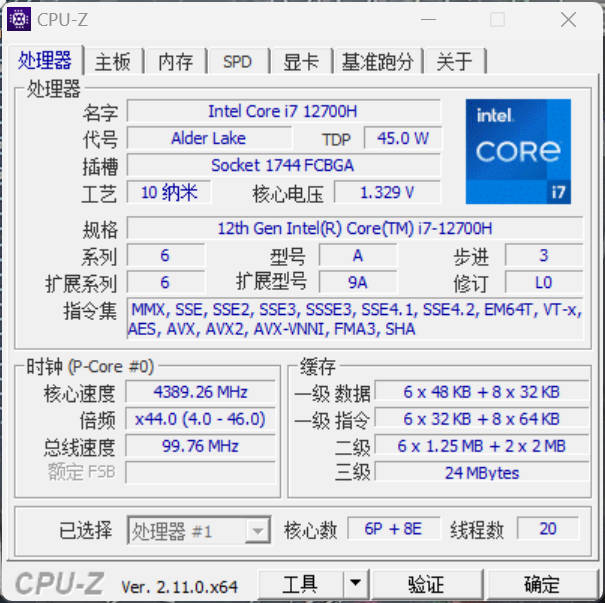
\includegraphics[width=0.8\textwidth]{fig/fig2}
    \end{figure}
\end{itemize}

\textbf{上述两组实验可以完成所提全部四种实验任务目标,原因如下:}
\begin{itemize}
    \item 实验1选择设置静态任务分配,固定粒度多粒度动态任务分配以及动态粒度动态任务分配,可以实现任务目标(1,2,4)
    \item 实验2选择动态粒度的动态任务分配,但设置多种线程规格对比可以实现任务目标(1,3)
\end{itemize}

\subsection{实验流程与结果分析}
\subsubsection{实验1代码实现}
首先引入相关库,并定义一些实验过程中所需的全局变量(如测试数组规模,重复测量次数等)。为了方便实验1中代码复用到实验2,这里我们将线程数定义为一个数组(当前只有一个4)。完整代码如下:
\begin{lstlisting}[language=C]
#include <omp.h>
#include <vector>
#include <algorithm>
#include <iostream>
#include <windows.h>
#include <random>
#include <ctime>

using namespace std;

const int ARR_NUM = 10000;  // 数组数量
const int ARR_LEN = 10000;  // 每个数组长度
const int REPEAT_TIMES = 10; // 每组测试重复次数

// 定义要测试的线程数数组
const vector<int> THREAD_NUMS = {4};  // 当前只使用4线程,后续可以方便地添加其他线程数

// 全局变量:存储初始的不均衡数组
vector<int> original_arrays[ARR_NUM];
\end{lstlisting}

随后我们考虑静态任务分配的代码实现。由于我们采用OpenMP编程,故相较于pthread此实现十分容易--只需在每一个数组的遍历的循环指定使用多线程对数组进行排序即可,代码如下:
\begin{lstlisting}[language=C]
// 使用静态调度的稳定排序函数
double test_static_scheduling(int num_threads) {
    vector<int> test_arrays[ARR_NUM];
    LARGE_INTEGER freq, start, end;
    QueryPerformanceFrequency(&freq);
    double total_time = 0.0;

    for (int t = 0; t < REPEAT_TIMES; t++) {
        copy_arrays(test_arrays);
        QueryPerformanceCounter(&start);

        #pragma omp parallel num_threads(num_threads)
        {
            #pragma omp for schedule(static)
            for (int i = 0; i < ARR_NUM; i++) {
                stable_sort(test_arrays[i].begin(), test_arrays[i].end());
            }
        }

        QueryPerformanceCounter(&end);
        total_time += (double)(end.QuadPart - start.QuadPart) * 1000.0 / freq.QuadPart;
    }

    return total_time / REPEAT_TIMES;
}
\end{lstlisting}

接着,我们考虑多粒度动态任务分配代码的实现,此步较为简单,只需将静态任务分配中schedule里面的static改成dynamic即可,同时指定每次任务分配的粒度。实现代码如下:
\begin{lstlisting}[language=C]
// 使用动态调度的稳定排序函数
double test_dynamic_scheduling(int chunk_size, int num_threads) {
    vector<int> test_arrays[ARR_NUM];
    LARGE_INTEGER freq, start, end;
    QueryPerformanceFrequency(&freq);
    double total_time = 0.0;

    for (int t = 0; t < REPEAT_TIMES; t++) {
        copy_arrays(test_arrays);
        QueryPerformanceCounter(&start);

        #pragma omp parallel num_threads(num_threads)
        {
            #pragma omp for schedule(dynamic, chunk_size)
            for (int i = 0; i < ARR_NUM; i++) {
                stable_sort(test_arrays[i].begin(), test_arrays[i].end());
            }
        }

        QueryPerformanceCounter(&end);
        total_time += (double)(end.QuadPart - start.QuadPart) * 1000.0 / freq.QuadPart;
    }

    return total_time / REPEAT_TIMES;
}
\end{lstlisting}

随后我们考虑动态粒度动态任务分配的实现,此步也只需将对应静态任务分配中的static字段改为guided即可,但在代码实现前让我们先熟悉一下guided的具体原理,如下:
\begin{itemize}
    \item 起始阶段,分配的任务块较大,以便迅速减少未完成的任务数量。
    \item 随着任务的完成,任务块逐渐减小,从而在后期更加细粒度地分配任务。
    \item 每个任务块的大小依据以下公式动态计算:
    \[
    S_k = \left\lceil \frac{R_k}{2N} \right\rceil
    \]
    其中:
    \begin{itemize}
        \item $S_k$ 表示第 $k$ 个分块的大小;
        \item $R_k$ 表示剩余任务的总量;
        \item $N$ 是线程的个数。
    \end{itemize}
    \item 这种策略兼顾了动态调度的灵活性和减少调度开销的目标。
\end{itemize}
与 \texttt{dynamic} 调度相比,\texttt{guided} 在工作负载不均匀时通常能提供更好的负载均衡。

在理解guided调度的原理后,我们进行相关代码的编写。相关代码如下

\begin{lstlisting}[language=C]
// 使用guided调度的稳定排序函数
double test_guided_scheduling(int num_threads) {
    vector<int> test_arrays[ARR_NUM];
    LARGE_INTEGER freq, start, end;
    QueryPerformanceFrequency(&freq);
    double total_time = 0.0;

    for (int t = 0; t < REPEAT_TIMES; t++) {
        copy_arrays(test_arrays);
        QueryPerformanceCounter(&start);

        #pragma omp parallel num_threads(num_threads)
        {
            #pragma omp for schedule(guided)
            for (int i = 0; i < ARR_NUM; i++) {
                stable_sort(test_arrays[i].begin(), test_arrays[i].end());
            }
        }

        QueryPerformanceCounter(&end);
        total_time += (double)(end.QuadPart - start.QuadPart) * 1000.0 / freq.QuadPart;
    }

    return total_time / REPEAT_TIMES;
}
\end{lstlisting}

最后是主函数的编写,这里完成相关类别任务测试代码编写的逻辑即可。具体代码如下:
\begin{lstlisting}[language=C]
int main() {
    cout << "Initializing original arrays..." << endl;
    init_original_arrays();

    cout << "Starting performance tests..." << endl;
    cout << fixed;
    cout.precision(3);

    // 对每个线程数进行测试
    for(int thread_count : THREAD_NUMS) {
        cout << "\nTesting with " << thread_count << " threads:" << endl;

        // 测试静态调度
        cout << "\nStatic scheduling test:" << endl;
        double static_time = test_static_scheduling(thread_count);
        cout << "Average time: " << static_time << " ms" << endl;

        // 测试不同粒度的动态调度
        cout << "\nDynamic scheduling tests:" << endl;
        // 1~100每间隔10测试(1~10间隔9)
        for (int chunk_size = 1; chunk_size <= 100; chunk_size += (chunk_size < 10 ? 9 : 10)) {
            double dynamic_time = test_dynamic_scheduling(chunk_size, thread_count);
            cout << "Chunk size " << chunk_size << ": " << dynamic_time << " ms" << endl;
        }
        // 100~1000每间隔100测试
        for (int chunk_size = 200; chunk_size <= 1000; chunk_size += 100) {
            double dynamic_time = test_dynamic_scheduling(chunk_size, thread_count);
            cout << "Chunk size " << chunk_size << ": " << dynamic_time << " ms" << endl;
        }

        // 测试guided调度
        cout << "\nGuided scheduling test:" << endl;
        double guided_time = test_guided_scheduling(thread_count);
        cout << "Average time: " << guided_time << " ms" << endl;
    }

    return 0;
}
\end{lstlisting}
至此,代码编写结束

\subsubsection{实验1结果与分析}
执行上述代码,我们获得实验结果如下(为了避免偶然误差,我们选择重复测试 10 次并取平均值)

\begin{table}[H]
\centering
\caption{各组实验 10 次测试中耗时最长线程所花费时间平均值}
\begin{tabular}{ccc}
\toprule
\textbf{Method} & \textbf{Block Size} & \textbf{Avg Max Thread Time (ms)} \\
\midrule
Static & - & 1879.472 \\
Dynamic & 1 & 1706.260 \\
Dynamic & 10 & 1714.684 \\
Dynamic & 20 & 1709.358 \\
Dynamic & 30 & 1722.447 \\
Dynamic & 40 & 1733.931 \\
Dynamic & 50 & 1726.078 \\
Dynamic & 60 & 2113.136 \\
Dynamic & 70 & 1826.351 \\
Dynamic & 80 & 2140.879 \\
Dynamic & 90 & 2109.537 \\
Dynamic & 100 & 2105.771 \\
Dynamic & 200 & 2180.800 \\
Dynamic & 300 & 2244.872 \\
Dynamic & 400 & 2344.049 \\
Dynamic & 500 & 2142.983 \\
Dynamic & 600 & 2360.087 \\
Dynamic & 700 & 2343.529 \\
Dynamic & 800 & 2415.492 \\
Dynamic & 900 & 2399.745 \\
Dynamic & 1000 & 2681.789 \\
Guided & - & 2203.573 \\
\bottomrule
\end{tabular}
\label{table:scheduling_results_detailed}
\end{table}

图像显示如下:
\begin{figure}[H]
\centering
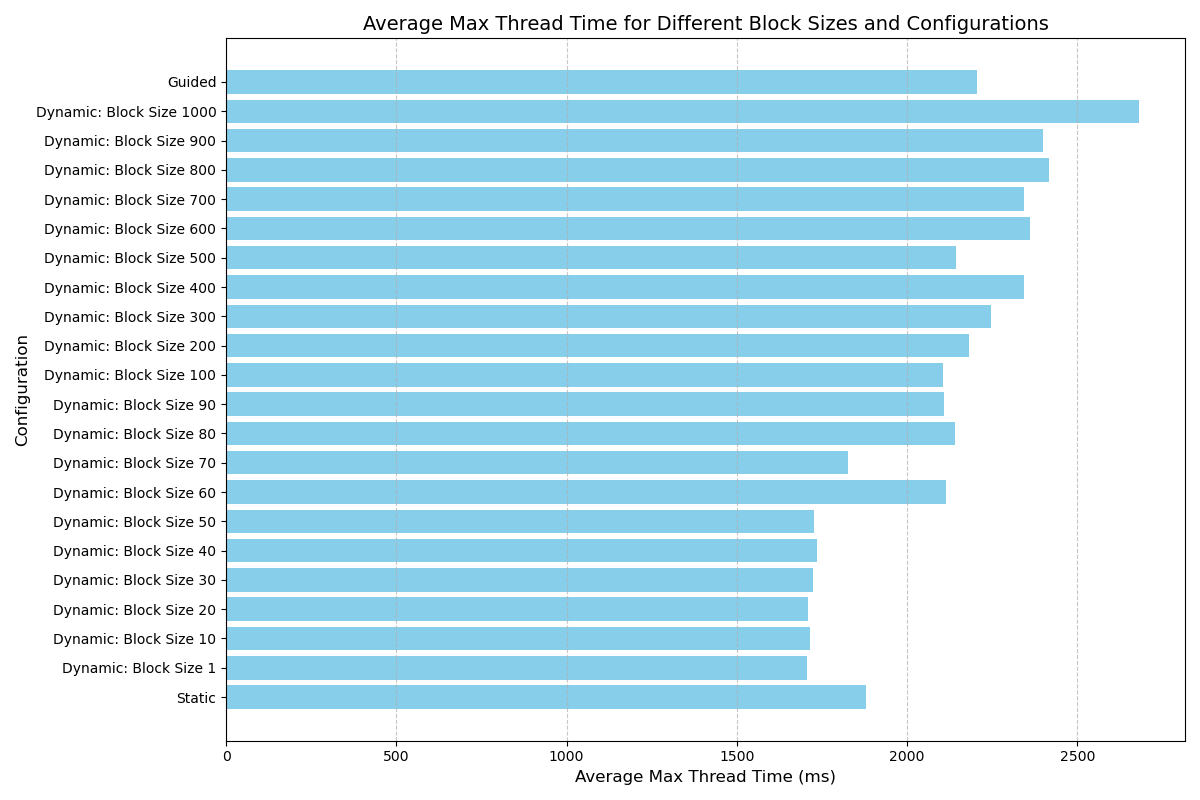
\includegraphics[width=0.8\textwidth]{fig/fig3.png}
\caption{各组实验10次测试中耗时平均值}
\end{figure}

由上图可见,当各数组排序难度不一致时较细粒度动态任务分配优于静态任务分配。同时动态粒度动态任务分配优于粗粒度动态任务分配。但是静态任务分配却优于粗粒度动态任务分配与动态粒度动态任务分配。

出现上述结果我们的分析如下:
\begin{enumerate}
    \item \textbf{较细粒度动态任务分配优于静态任务分配:}推测原因为为负载不均衡问题的解决
    \begin{itemize}
        \item 在粗粒度动态任务分配中,任务粒度较大,某些线程可能会被分配到复杂任务,而其他线程分配到简单任务,仍可能出现线程空闲或任务分布不均的情况。但动态粒度动态任务分配通过更小的任务粒度(例如单个数组或部分数组片段)动态分配任务,使得任务调度更加灵活,显著提高了线程的并行效率。
    \end{itemize}
    \item \textbf{细粒度动态任务分配优于粗粒度动态任务分配:}推测原因为为任务分配的灵活性
    \begin{itemize}
        \item 粗粒度动态分配虽然能一定程度解决负载不均问题,但任务粒度较大时,单个线程分配到复杂任务后仍可能成为性能瓶颈,导致其它线程等待。 细粒度动态分配通过将任务划分得更小,显著提升了任务调度的灵活性,使线程能快速切换到新的任务上,进一步减少了线程闲置时间。
    \end{itemize}
    \item \textbf{静态任务分配优于粗粒度和动态粒度动态任务分配:}推测原因为调度开销的影响与线程缓存效应
    \begin{itemize}
        \item 调度开销的影响:动态分配相比静态分配需要在运行时动态调度任务,每次调度都引入了一定的系统开销。如果任务粒度较粗,任务数量较少,则动态调度的开销可能抵消其带来的负载均衡优势。
        \item 线程缓存效应:静态任务分配由于任务的分配是固定的,线程可以更好地利用数据的局部性和缓存效果。而动态分配可能因为任务分布的不确定性导致线程间缓存竞争,从而影响性能。
    \end{itemize}
    \item \textbf{动态粒度动态任务分配优于粗粒度动态任务分配:}推测原因为:任务拆分更细,提升资源利用率,使得负载平衡效果明显
    \begin{itemize}
        \item 在粗粒度动态任务分配中,任务粒度较大,线程容易因负载不均而导致资源浪费。而动态粒度任务分配通过细化任务粒度,能够更均匀地分配负载,减少线程等待和空闲时间。而动态粒度任务分配的高频调度虽然增加了一些开销,但这种方式能快速将剩余任务分配给空闲线程,在负载不均的情况下极大地提高了整体运行效率。
    \end{itemize}
\end{enumerate}

由上述分析我们得出以下总结:
\begin{enumerate}
    \item \textbf{排序难度差异的作用}\\
    排序任务的复杂性差异对实验结果有直接影响。复杂任务的执行时间较长,而简单任务执行时间短,导致线程之间负载不均。在这种情况下,各分配策略表现如下:
    \begin{itemize}
        \item \textbf{静态任务分配:}由于任务分配在编译时固定,高负载任务可能集中分配到部分线程,导致其他线程完成任务后出现长时间的空闲,资源利用率低,整体表现较差。
        \item \textbf{粗粒度动态任务分配:}虽然粗粒度动态任务分配能够一定程度缓解负载不均,但任务粒度较大,部分线程仍可能分配到复杂任务,导致负载差异无法彻底解决,性能提升有限。
        \item \textbf{动态粒度动态任务分配:}通过调整粒度,动态粒度动态任务分配将任务划分得比粗粒度更细,可以更好地平衡负载。然而,由于调度粒度较细,调度开销增加,性能的提升依赖于任务划分的合理性。
        \item \textbf{细粒度动态任务分配:}将任务划分得更小,细粒度动态任务分配能有效地将任务动态分配到空闲线程中,显著改善负载分布不均的问题,线程利用率更高。
    \end{itemize}
    \item \textbf{动态任务分配的优越性}\\
    动态任务分配的核心优势在于其灵活性,尤其是在任务负载高度不均的情况下。动态粒度和细粒度的动态任务分配相比静态和粗粒度分配,表现出以下特点:
    \begin{itemize}
        \item \textbf{动态粒度动态任务分配:}通过适当细化任务粒度,在减少负载不均的同时,将调度开销控制在合理范围内。这种平衡使其在大多数场景下表现优于粗粒度分配。
        \item \textbf{细粒度动态任务分配:}虽然调度的开销较高,但在排序负载差异显著的情况下,细粒度任务分配通过高度灵活的调度,显著提升了线程资源利用率。调度带来的负载均衡收益远大于开销,使得其整体性能优于其他分配策略。
    \end{itemize}
\end{enumerate}

因此在负载差异大的排序任务中,动态任务分配策略可提升效率,而分配粒度的选择则是性能优化的关键。一方面,过大的任务粒度可能导致负载不均衡,影响性能;另一方面,过小的任务粒度则会带来额外的调度开销,可能抵消负载均衡带来的收益。因此,在具体场景中,需要根据任务的负载差异和计算规模,合理地调整任务粒度,找到调度开销与负载均衡之间的最佳平衡点。只有在这一点上达成优化,动态任务分配才能发挥其最大的性能提升作用。

\subsubsection{试验2代码编写}
由于实验2所需代码与实验1中代码高度重合,仅部分变量设定不同,这里我们仅给出实验2相较于实验1中代码的不同部分:

首先时线程数量设置,这里我们选择将其设置为2$\sim$20,每间隔2,具体如下:
\begin{lstlisting}[language=C]
// 定义要测试的线程数数组
const vector<int> THREAD_NUMS = {2,4,6,8,10,12,14,16,18,20};  // 实验1则设定为const vector<int> THREAD_NUMS = {4}即可
\end{lstlisting}

随后是主函数代码编写,这里编写也较为简单,只需保留实验1中guided的测试部分并在每组实验输出当前线程数即可。对应代码如下:
\begin{lstlisting}[language=C]
int main() {
    cout << "Initializing original arrays..." << endl;
    init_original_arrays();

    cout << "Starting performance tests..." << endl;
    cout << fixed;
    cout.precision(3);

    // 对每个线程数进行测试
    for(int thread_count : THREAD_NUMS) {
        /*cout << "\nTesting with " << thread_count << " threads:" << endl;

        // 测试静态调度
        cout << "\nStatic scheduling test:" << endl;
        double static_time = test_static_scheduling(thread_count);
        cout << "Average time: " << static_time << " ms" << endl;

        // 测试不同粒度的动态调度
        cout << "\nDynamic scheduling tests:" << endl;
        // 1~100每间隔10测试(1~10间隔9)
        for (int chunk_size = 1; chunk_size <= 100; chunk_size += (chunk_size < 10 ? 9 : 10)) {
            double dynamic_time = test_dynamic_scheduling(chunk_size, thread_count);
            cout << "Chunk size " << chunk_size << ": " << dynamic_time << " ms" << endl;
        }
        // 100~1000每间隔100测试
        for (int chunk_size = 200; chunk_size <= 1000; chunk_size += 100) {
            double dynamic_time = test_dynamic_scheduling(chunk_size, thread_count);
            cout << "Chunk size " << chunk_size << ": " << dynamic_time << " ms" << endl;
        }实验1则取消注释此段*/

        // 测试guided调度
        cout << "\nGuided scheduling test of "<<thread_count<<" threads" << endl;
        double guided_time = test_guided_scheduling(thread_count);
        cout << "Average time: " << guided_time << " ms" << endl;
    }

    return 0;
}
\end{lstlisting}
至此,代码编写结束。

\subsubsection{试验2结果与分析}
获得实验结果如下:
\begin{table}[H]
\centering
\caption{Guided Scheduling Test Results}
\begin{tabular}{cc}
\toprule
\textbf{Number of Threads} & \textbf{Average Time (ms)} \\
\midrule
2  & 3069.448 \\
4  & 1649.231 \\
6  & 1172.097 \\
8  & 969.277 \\
10 & 856.627 \\
12 & 781.024 \\
14 & 730.718 \\
16 & 692.552 \\
18 & 637.809 \\
20 & 595.742 \\
\bottomrule
\end{tabular}
\label{table:guided-scheduling-new}
\end{table}


图像显示如下:
\begin{figure}[H]
\centering
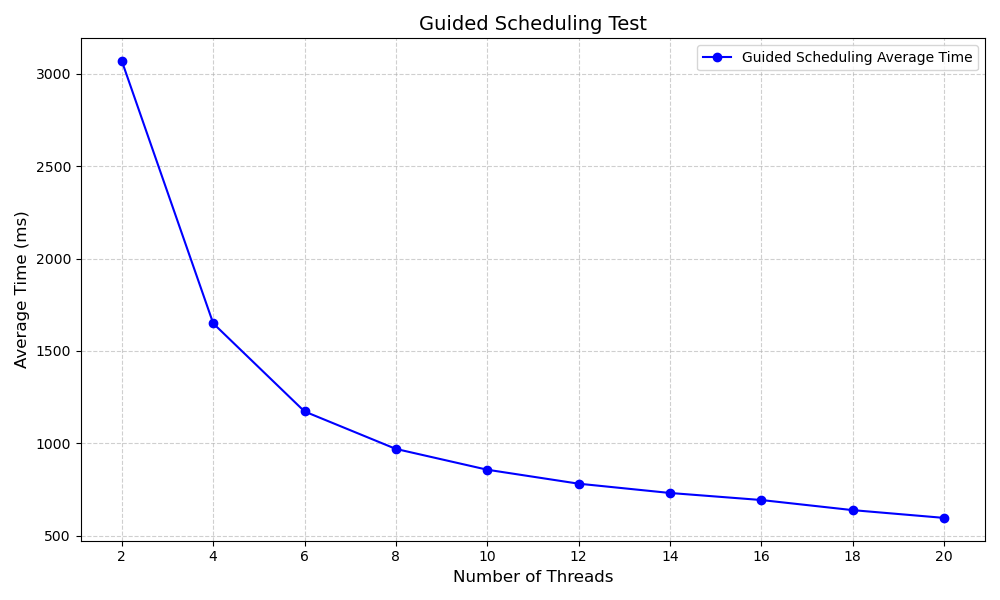
\includegraphics[width=0.8\textwidth]{fig/fig4.png}
\caption{实验2运行时间比较图}
\end{figure}

由上图可见,当我们采用固定的任务分配机制时。在我们所设定的线程范围内,程序运行时间随着线程数量的增加而减少,并且开始时时间减少较快,随着线程数量的增加,这种减少变得愈发不明显。但总体上仍呈现随着线程增加运行时间减少的趋势。以下是对出现此现象的分析:
\begin{itemize}
    \item 当采用固定的任务分配机制时,每个线程的负载会根据线程数量的不同而变化。在并行计算中,当线程数量增加时,每个线程可以分配到更少的任务,因此总体的执行时间会减少。但是,线程数量的增加并不总是能线性地减少执行时间,尤其是在线程数达到一定规模之后。
    \item 在并行计算中,线程的创建、调度和上下文切换是有成本的。当线程数量较少时,这些开销相对较小,因此增加线程数能有效地加速计算。但当线程数过多时,线程调度和管理的开销会变得更加显著,导致并行加速效应减弱。
    \item Amdahl’s Law 描述了并行计算中加速比的限制。当一个程序中的某些部分是串行执行的,即使增加了大量的线程,只有部分工作可以并行化。随着线程数量的增加,更多的时间被消耗在串行部分上,导致加速效果减小,最终并没有线性地缩短运行时间。因此,在某些情形下,线程数增加到一定程度后,性能提升变得不明显,甚至可能出现性能下降。
    \item 当线程数增多时,可能会出现缓存和内存带宽的瓶颈。如果每个线程需要频繁访问共享数据或大规模的内存操作,可能会导致缓存未命中和内存带宽不足,从而降低性能。这种情况下,线程数的增加可能会引起系统负载的过度增加,从而使得性能提升减缓。
    \item 线程数增加到一定程度后,程序的加速效应会趋于饱和。此时,增加更多的线程并不能有效提高性能,甚至可能因为过度的线程调度和同步开销导致性能下降。在这种情况下,程序的运行时间虽然依然呈现下降趋势,但下降幅度变得越来越小,最终趋于平稳。
\end{itemize}

因此,在选择合适的线程数时,不仅要考虑计算任务的并行度,还要充分考虑线程调度、同步、缓存和内存带宽等因素,避免线程数过少而导致程序运行时间过少,但也要避免线程数过多导致的性能瓶颈。

至此,本实验结束。

\subsection{思考总结}
在这次实验中,我深入探索了OpenMP在处理多个数组排序任务中的应用,尤其是针对任务不均衡问题的解决方案。通过实验,我对并行计算中的任务调度策略有了更深刻的理解。

首先,实验让我意识到任务分配策略对并行程序性能的影响是多么显著。静态任务分配虽然简单,但在负载不均的情况下,容易导致某些线程过载,而其他线程则可能闲置。相比之下,动态任务分配,尤其是细粒度的动态任务分配,能够更好地平衡负载,显著提高线程的利用率。

其次,实验中使用的guided调度策略让我感受到其在负载不均情况下的优势。通过动态调整任务块的大小,guided调度在减少调度开销的同时,能够更灵活地分配任务,提升了整体性能。这种策略的灵活性和高效性在实验结果中得到了验证。

此外,实验还让我重新审视了线程数对程序性能的影响。虽然增加线程数通常能加速计算,但过多的线程可能导致调度开销增加,甚至出现性能瓶颈。这让我意识到,在并行编程中,选择合适的线程数是一个需要仔细权衡的决策。

总的来说,这次实验不仅让我掌握了OpenMP的基本用法,还让我对并行计算中的任务调度策略有了更深刻的理解。未来,我希望能将这些经验应用到更复杂的并行计算任务中,进一步提升程序的性能和效率。

\section{高斯消去法的OpenMP实现,并与SSE/AVX编程结合探索优化任务分配方法}
\subsection{实验目的}
实现高斯消去法解线性方程组的OpenMP编程,与SSE/AVX编程结合,并探索优化任务分配方法。

\subsection{实验要求}
\begin{enumerate}
    \item 问题描述
    \item 算法设计和实现
    \item 实验及结果分析
\end{enumerate}

\subsection{问题描述}
本实验旨在深入理解并实现高斯消元法用于求解线性方程组的OpenMP版本,并与SSE/AVX编程相结合,探索规律。任务分为以下步骤:
\begin{enumerate}
    \item \textbf{高斯消元法学习:}首先熟悉高斯消元法的理论和步骤,包括消元阶段和回代阶段的具体流程。
    \item \textbf{OpenMP版本高斯消元实现:}在单线程实现的基础上,利用OpenMP编写多线程版本的高斯消元法,通过并行化加速消元和回代过程。
    \item \textbf{结合 SSE/AVX 指令优化:}在关键计算部分(如浮点数计算)加入 SSE/AVX 指令集,以实现更高效的矢量化计算。
    \item \textbf{任务分配优化:}研究并实现优化的任务分配策略,将计算任务合理分配到不同线程中,进一步提高算法的整体执行效率。
\end{enumerate}

\subsection{对高斯消元法的理解}
\textbf{原理}

考虑线性方程组:
\begin{equation}
    \begin{cases}
    a_{11}x_1 + a_{12}x_2 + \cdots + a_{1n}x_n = b_1 \\
    a_{21}x_1 + a_{22}x_2 + \cdots + a_{2n}x_n = b_2 \\
    \vdots \\
    a_{n1}x_1 + a_{n2}x_2 + \cdots + a_{nn}x_n = b_n
    \end{cases}
\end{equation}

其增广矩阵为:
\begin{equation}
    \left[
    \begin{array}{cccc|c}
    a_{11} & a_{12} & \cdots & a_{1n} & b_1 \\
    a_{21} & a_{22} & \cdots & a_{2n} & b_2 \\
    \vdots & \vdots & \ddots & \vdots & \vdots \\
    a_{n1} & a_{n2} & \cdots & a_{nn} & b_n
    \end{array}
    \right]
\end{equation}

\textbf{算法步骤}
\begin{algorithm}[H]
    \caption{高斯消元法}
    \label{alg:gaussian-elimination}
    \begin{algorithmic}
    \STATE 1. 前向消元(化上三角):
    \FOR{$k = 1$ to $n-1$}
        \FOR{$i = k+1$ to $n$}
            \STATE 计算乘数:$m_{ik} = a_{ik}/a_{kk}$
            \FOR{$j = k+1$ to $n$}
                \STATE $a_{ij} = a_{ij} - m_{ik}a_{kj}$
            \ENDFOR
            \STATE $b_i = b_i - m_{ik}b_k$
        \ENDFOR
    \ENDFOR
    \STATE 2. 回代求解:
    \STATE $x_n = b_n/a_{nn}$
    \FOR{$i = n-1$ down to $1$}
        \STATE $sum = 0$
        \FOR{$j = i+1$ to $n$}
            \STATE $sum = sum + a_{ij}x_j$
        \ENDFOR
        \STATE $x_i = (b_i - sum)/a_{ii}$
    \ENDFOR
    \end{algorithmic}
\end{algorithm}

\textbf{可知,该算法时间复杂度为$O(n^3)$}

\subsection{实验设计}
\subsubsection{实验环境}
\begin{itemize}
    \item \textbf{CPU:}Intel Core i7 12700H
    \item \textbf{操作系统:}Windows
    \item \textbf{编译器:}TDM-GCC 10.3.0
    \item \textbf{IDE:}Code::Blocks 20.03
\end{itemize}

\subsubsection{实验数据及方法设置}
\begin{enumerate}[label=\arabic*.]
    \item 测试矩阵大小:10$\times$10到1000$\times$1000。其中10到100每间隔10,100到1000每间隔100
    \item 每种算法对每种规模矩阵进行多次测试取平均值。同时,自动调整重复次数,确保总执行时间在10s左右且重复次数不超10000
    \item 使用Windows高精度计时器QueryPerformance系列API测量执行用时
\end{enumerate}

\subsubsection{实验分组设置}
仅设置一组实验,但这一组实验中包含以下几种高斯消元法:
\begin{enumerate}
    \item 单线程未使用优化版本的高斯消元法
    \item 基于OpenMP的多线程未使用优化版本的高斯消元法(静态任务分配)
    \item 基于OpenMP的多线程未使用优化版本的高斯消元法(动态任务分配)
    \item 单线程使用SSE优化版本的高斯消元法
    \item 基于OpenMP的多线程使用SSE优化版本的高斯消元法(静态任务分配)
    \item 基于OpenMP的多线程使用SSE优化版本的高斯消元法(动态任务分配)
    \item 单线程使用AVX优化版本的高斯消元法
    \item 基于OpenMP的多线程使用AVX优化版本的高斯消元法(静态任务分配)
    \item 基于OpenMP的多线程使用AVX优化版本的高斯消元法(动态任务分配)
\end{enumerate}

请注意,我们设定多线程版本中线程数为4。同时,动态任务分配中分配任务的粒度大小为1

\subsection{实验流程与结果分析}
\subsubsection{实验代码实现}
首先引入相关库,。同时,参考上次高斯消元法相关测试函数(如生成测试矩阵以及时间测量等)。代码如下:
\begin{lstlisting}[language=C]
#include <iostream>
#include <vector>
#include <chrono>
#include <random>
#include <iomanip>
#include <windows.h>
#include <immintrin.h>
#include <omp.h>
#include <cmath>

using namespace std;

// 计时函数
inline double get_time() {
    LARGE_INTEGER freq, counter;
    QueryPerformanceFrequency(&freq);
    QueryPerformanceCounter(&counter);
    return static_cast<double>(counter.QuadPart) / freq.QuadPart;
}

// 内存分配函数
float** allocate_matrix(int n) {
    float** matrix = new float*[n];
    for (int i = 0; i < n; i++) {
        matrix[i] = new float[n];
    }
    return matrix;
}

void free_matrix(float** matrix, int n) {
    for (int i = 0; i < n; i++) {
        delete[] matrix[i];
    }
    delete[] matrix;
}

// 矩阵生成函数
void generate_random_matrix(float** A, float* b, int n) {
    random_device rd;
    mt19937 gen(rd());
    uniform_real_distribution<float> dis(1.0f, 100.0f);

    for (int i = 0; i < n; i++) {
        for (int j = 0; j < n; j++) {
            A[i][j] = dis(gen);
        }
        b[i] = dis(gen);
    }
}

// 数据复制函数
void copy_data(float** dst_A, float* dst_b, float** src_A, float* src_b, int n) {
    for (int i = 0; i < n; i++) {
        for (int j = 0; j < n; j++) {
            dst_A[i][j] = src_A[i][j];
        }
        dst_b[i] = src_b[i];
    }
}
\end{lstlisting}

随后实现基础串行版本的高斯消元法,基础 SSE 版本的高斯消元法,基础 AVX 版本的高斯消元法,由于上次实验中以及实现,故这里不再赘述,仅给出相应代码,代码如下:
\begin{lstlisting}[language=C]
// 回代过程(串行)
void back_substitution(float** A, float* b, float* x, int n) {
    for (int i = n - 1; i >= 0; i--) {
        float sum = 0;
        for (int j = i + 1; j < n; j++) {
            sum += A[i][j] * x[j];
        }
        x[i] = (b[i] - sum) / A[i][i];
    }
}

// 普通串行高斯消元
void serial_solver(int n, float** A, float* b, float* x) {
    for (int k = 0; k < n; k++) {
        for (int i = k + 1; i < n; i++) {
            float factor = A[i][k] / A[k][k];
            for (int j = k; j < n; j++) {
                A[i][j] -= factor * A[k][j];
            }
            b[i] -= factor * b[k];
        }
    }
    back_substitution(A, b, x, n);
}

// SSE优化的回代过程
void back_substitution_sse(float** A, float* b, float* x, int n) {
    x[n-1] = b[n-1] / A[n-1][n-1];

    for (int i = n - 2; i >= 0; i--) {
        __m128 sum = _mm_setzero_ps();
        int j = i + 1;

        for (; j + 4 <= n; j += 4) {
            __m128 a = _mm_loadu_ps(&A[i][j]);
            __m128 xv = _mm_loadu_ps(&x[j]);
            sum = _mm_add_ps(sum, _mm_mul_ps(a, xv));
        }

        float sum_array[4];
        _mm_storeu_ps(sum_array, sum);
        float final_sum = sum_array[0] + sum_array[1] + sum_array[2] + sum_array[3];

        for (; j < n; j++) {
            final_sum += A[i][j] * x[j];
        }

        x[i] = (b[i] - final_sum) / A[i][i];
    }
}

// SSE单线程优化版本
void gaussian_elimination_sse_all(int n, float** A, float* b, float* x) {
    for (int k = 0; k < n; k++) {
        for (int i = k + 1; i < n; i++) {
            float factor = A[i][k] / A[k][k];
            __m128 factor4 = _mm_set1_ps(factor);

            int j;
            for (j = k; j + 4 <= n; j += 4) {
                __m128 mk = _mm_loadu_ps(&A[k][j]);
                __m128 mi = _mm_loadu_ps(&A[i][j]);
                __m128 result = _mm_sub_ps(mi, _mm_mul_ps(factor4, mk));
                _mm_storeu_ps(&A[i][j], result);
            }
            for (; j < n; j++) {
                A[i][j] -= factor * A[k][j];
            }
            b[i] -= factor * b[k];
        }
    }
    back_substitution_sse(A, b, x, n);
}

// AVX优化的回代过程
void back_substitution_avx(float** A, float* b, float* x, int n) {
    x[n-1] = b[n-1] / A[n-1][n-1];

    for (int i = n - 2; i >= 0; i--) {
        __m256 sum = _mm256_setzero_ps();
        int j = i + 1;

        for (; j + 8 <= n; j += 8) {
            __m256 a = _mm256_loadu_ps(&A[i][j]);
            __m256 xv = _mm256_loadu_ps(&x[j]);
            sum = _mm256_add_ps(sum, _mm256_mul_ps(a, xv));
        }

        float sum_array[8];
        _mm256_storeu_ps(sum_array, sum);
        float final_sum = sum_array[0] + sum_array[1] + sum_array[2] + sum_array[3] +
                         sum_array[4] + sum_array[5] + sum_array[6] + sum_array[7];

        for (; j < n; j++) {
            final_sum += A[i][j] * x[j];
        }

        x[i] = (b[i] - final_sum) / A[i][i];
    }
}

// AVX单线程优化版本
void gaussian_elimination_avx_all(int n, float** A, float* b, float* x) {
    for (int k = 0; k < n; k++) {
        for (int i = k + 1; i < n; i++) {
            float factor = A[i][k] / A[k][k];
            __m256 factor8 = _mm256_set1_ps(factor);

            int j;
            for (j = k; j + 8 <= n; j += 8) {
                __m256 mk = _mm256_loadu_ps(&A[k][j]);
                __m256 mi = _mm256_loadu_ps(&A[i][j]);
                __m256 result = _mm256_sub_ps(mi, _mm256_mul_ps(factor8, mk));
                _mm256_storeu_ps(&A[i][j], result);
            }
            for (; j < n; j++) {
                A[i][j] -= factor * A[k][j];
            }
            b[i] -= factor * b[k];
        }
    }
    back_substitution_avx(A, b, x, n);
}
\end{lstlisting}

接下来,分别是基础版本、SSE 版本、AVX 版本的基于OpenMP的多线程静态任务分配。在这里我们设定为 4 个线程。故每个线程只需要完成一次任务中$\frac{1}{4}$的任务量即可,考虑到相应数值依赖关系,这里的多线程只能在
高斯消元算法最外层循环内部进行多线程操作(下述多线程同理)。相应代码如下:
\begin{lstlisting}[language=C]
// OpenMP静态调度版本
void gaussian_elimination_static_omp(int n, float** A, float* b, float* x) {
    omp_set_num_threads(4);  // 设置使用4个线程
    for (int k = 0; k < n; k++) {
        #pragma omp parallel for schedule(static)
        for (int i = k + 1; i < n; i++) {
            float factor = A[i][k] / A[k][k];
            for (int j = k; j < n; j++) {
                A[i][j] -= factor * A[k][j];
            }
            b[i] -= factor * b[k];
        }
    }
    back_substitution_sse(A, b, x, n);
}

// OpenMP + SSE静态调度版本
void gaussian_elimination_sse_static_omp(int n, float** A, float* b, float* x) {
    omp_set_num_threads(4);  // 设置使用4个线程
    for (int k = 0; k < n; k++) {
        #pragma omp parallel for schedule(static)
        for (int i = k + 1; i < n; i++) {
            float factor = A[i][k] / A[k][k];
            __m128 factor4 = _mm_set1_ps(factor);

            int j;
            for (j = k; j + 4 <= n; j += 4) {
                __m128 mk = _mm_loadu_ps(&A[k][j]);
                __m128 mi = _mm_loadu_ps(&A[i][j]);
                __m128 result = _mm_sub_ps(mi, _mm_mul_ps(factor4, mk));
                _mm_storeu_ps(&A[i][j], result);
            }
            for (; j < n; j++) {
                A[i][j] -= factor * A[k][j];
            }
            b[i] -= factor * b[k];
        }
    }
    back_substitution_sse(A, b, x, n);
}

// OpenMP + AVX静态调度版本
void gaussian_elimination_avx_static_omp(int n, float** A, float* b, float* x) {
    omp_set_num_threads(4);  // 设置使用4个线程
    for (int k = 0; k < n; k++) {
        #pragma omp parallel for schedule(static)
        for (int i = k + 1; i < n; i++) {
            float factor = A[i][k] / A[k][k];
            __m256 factor8 = _mm256_set1_ps(factor);

            int j;
            for (j = k; j + 8 <= n; j += 8) {
                __m256 mk = _mm256_loadu_ps(&A[k][j]);
                __m256 mi = _mm256_loadu_ps(&A[i][j]);
                __m256 result = _mm256_sub_ps(mi, _mm256_mul_ps(factor8, mk));
                _mm256_storeu_ps(&A[i][j], result);
            }
            for (; j < n; j++) {
                A[i][j] -= factor * A[k][j];
            }
            b[i] -= factor * b[k];
        }
    }
    back_substitution_avx(A, b, x, n);
}
\end{lstlisting}

然后,分别是基础版本、SSE 版本、AVX 版本的动态任务分配,这里我们设置每次任务分配的粒
度为 1(以便测试不同规格的矩阵,使其具有鲁棒性),相应代码如下:
\begin{lstlisting}[language=C]
// OpenMP动态调度版本
void gaussian_elimination_dynamic_omp(int n, float** A, float* b, float* x) {
    omp_set_num_threads(4);  // 设置使用4个线程
    for (int k = 0; k < n; k++) {
        #pragma omp parallel for schedule(dynamic,1)
        for (int i = k + 1; i < n; i++) {
            float factor = A[i][k] / A[k][k];
            for (int j = k; j < n; j++) {
                A[i][j] -= factor * A[k][j];
            }
            b[i] -= factor * b[k];
        }
    }
    back_substitution_avx(A, b, x, n);
}

// OpenMP + SSE动态调度版本
void gaussian_elimination_sse_dynamic_omp(int n, float** A, float* b, float* x) {
    omp_set_num_threads(4);  // 设置使用4个线程
    for (int k = 0; k < n; k++) {
        #pragma omp parallel for schedule(dynamic,1)
        for (int i = k + 1; i < n; i++) {
            float factor = A[i][k] / A[k][k];
            __m128 factor4 = _mm_set1_ps(factor);

            int j;
            for (j = k; j + 4 <= n; j += 4) {
                __m128 mk = _mm_loadu_ps(&A[k][j]);
                __m128 mi = _mm_loadu_ps(&A[i][j]);
                __m128 result = _mm_sub_ps(mi, _mm_mul_ps(factor4, mk));
                _mm_storeu_ps(&A[i][j], result);
            }
            for (; j < n; j++) {
                A[i][j] -= factor * A[k][j];
            }
            b[i] -= factor * b[k];
        }
    }
    back_substitution_sse(A, b, x, n);
}

// OpenMP + AVX动态调度版本
void gaussian_elimination_avx_dynamic_omp(int n, float** A, float* b, float* x) {
    omp_set_num_threads(4);  // 设置使用4个线程
    for (int k = 0; k < n; k++) {
        #pragma omp parallel for schedule(dynamic,1)
        for (int i = k + 1; i < n; i++) {
            float factor = A[i][k] / A[k][k];
            __m256 factor8 = _mm256_set1_ps(factor);

            int j;
            for (j = k; j + 8 <= n; j += 8) {
                __m256 mk = _mm256_loadu_ps(&A[k][j]);
                __m256 mi = _mm256_loadu_ps(&A[i][j]);
                __m256 result = _mm256_sub_ps(mi, _mm256_mul_ps(factor8, mk));
                _mm256_storeu_ps(&A[i][j], result);
            }
            for (; j < n; j++) {
                A[i][j] -= factor * A[k][j];
            }
            b[i] -= factor * b[k];
        }
    }
    back_substitution_avx(A, b, x, n);
}
\end{lstlisting}

接下来是相应测试函数,以完成重复测试多次但总时间10s左右,总测试次数不超过10000次。相应代码如下:
\begin{lstlisting}[language=C]
// 测试函数
void benchmark_solver(const string& name, void (*solver)(int, float**, float*, float*),
                     float** A, float* b, float* x, int n, int& repeat_count) {
    double total_time = 0;
    float** temp_A = allocate_matrix(n);
    float* temp_b = new float[n];

    // 预热运行
    copy_data(temp_A, temp_b, A, b, n);
    solver(n, temp_A, temp_b, x);

    // 确定重复次数
    copy_data(temp_A, temp_b, A, b, n);
    double start_time = get_time();
    solver(n, temp_A, temp_b, x);
    double single_time = get_time() - start_time;

    repeat_count = min(10000, max(1, int(10.0 / single_time)));

    // 实际测试
    for (int i = 0; i < repeat_count; i++) {
        copy_data(temp_A, temp_b, A, b, n);
        start_time = get_time();
        solver(n, temp_A, temp_b, x);
        total_time += get_time() - start_time;
    }

    cout << fixed << setprecision(6) << name << "," << n << ","
         << total_time << "," << repeat_count << "," << fixed << setprecision(9) << total_time / repeat_count << endl;

    free_matrix(temp_A, n);
    delete[] temp_b;
}
\end{lstlisting}

最后是主函数,在这里完成各组相应测试逻辑的编写,相应代码如下:
\begin{lstlisting}[language=C]
int main() {
    cout << "Algorithm,Size,Total Time(s),Repeats,Avg Time(s)" << endl;
    vector<int> sizes;

    // 生成测试规模
    for (int n = 10; n <= 100; n += 10) sizes.push_back(n);
    for (int n = 200; n <= 1000; n += 100) sizes.push_back(n);

    // 测试 "Serial" 版本
    for (int n : sizes) {
        float** A = allocate_matrix(n);
        float* b = new float[n];
        float* x = new float[n];
        int repeat_count;

        generate_random_matrix(A, b, n);
        benchmark_solver("Serial", serial_solver, A, b, x, n, repeat_count);

        free_matrix(A, n);
        delete[] b;
        delete[] x;
    }

    // 测试 "Static_OpenMP" 版本
    for (int n : sizes) {
        float** A = allocate_matrix(n);
        float* b = new float[n];
        float* x = new float[n];
        int repeat_count;

        generate_random_matrix(A, b, n);
        benchmark_solver("Static_OpenMP", gaussian_elimination_static_omp, A, b, x, n, repeat_count);

        free_matrix(A, n);
        delete[] b;
        delete[] x;
    }

    // 测试 "Dynamic_OpenMP" 版本
    for (int n : sizes) {
        float** A = allocate_matrix(n);
        float* b = new float[n];
        float* x = new float[n];
        int repeat_count;

        generate_random_matrix(A, b, n);
        benchmark_solver("Dynamic_OpenMP", gaussian_elimination_dynamic_omp, A, b, x, n, repeat_count);

        free_matrix(A, n);
        delete[] b;
        delete[] x;
    }

    // 测试 "SSE" 版本
    for (int n : sizes) {
        float** A = allocate_matrix(n);
        float* b = new float[n];
        float* x = new float[n];
        int repeat_count;

        generate_random_matrix(A, b, n);
        benchmark_solver("SSE", gaussian_elimination_sse_all, A, b, x, n, repeat_count);

        free_matrix(A, n);
        delete[] b;
        delete[] x;
    }

    // 测试 "SSE_OpenMP+Static" 版本
    for (int n : sizes) {
        float** A = allocate_matrix(n);
        float* b = new float[n];
        float* x = new float[n];
        int repeat_count;

        generate_random_matrix(A, b, n);
        benchmark_solver("SSE_OpenMP+Static", gaussian_elimination_sse_static_omp, A, b, x, n, repeat_count);

        free_matrix(A, n);
        delete[] b;
        delete[] x;
    }

    // 测试 "SSE_OpenMP+Dynamic" 版本
    for (int n : sizes) {
        float** A = allocate_matrix(n);
        float* b = new float[n];
        float* x = new float[n];
        int repeat_count;

        generate_random_matrix(A, b, n);
        benchmark_solver("SSE_OpenMP+Dynamic", gaussian_elimination_sse_dynamic_omp, A, b, x, n, repeat_count);

        free_matrix(A, n);
        delete[] b;
        delete[] x;
    }

    // 测试 "AVX" 版本
    for (int n : sizes) {
        float** A = allocate_matrix(n);
        float* b = new float[n];
        float* x = new float[n];
        int repeat_count;

        generate_random_matrix(A, b, n);
        benchmark_solver("AVX", gaussian_elimination_avx_all, A, b, x, n, repeat_count);

        free_matrix(A, n);
        delete[] b;
        delete[] x;
    }

    // 测试 "AVX_OpenMP+Static" 版本
    for (int n : sizes) {
        float** A = allocate_matrix(n);
        float* b = new float[n];
        float* x = new float[n];
        int repeat_count;

        generate_random_matrix(A, b, n);
        benchmark_solver("AVX_OpenMP+Static", gaussian_elimination_avx_static_omp, A, b, x, n, repeat_count);

        free_matrix(A, n);
        delete[] b;
        delete[] x;
    }

    // 测试 "AVX_OpenMP+Dynamic" 版本
    for (int n : sizes) {
        float** A = allocate_matrix(n);
        float* b = new float[n];
        float* x = new float[n];
        int repeat_count;

        generate_random_matrix(A, b, n);
        benchmark_solver("AVX_OpenMP+Dynamic", gaussian_elimination_avx_dynamic_omp, A, b, x, n, repeat_count);

        free_matrix(A, n);
        delete[] b;
        delete[] x;
    }

    return 0;
}
\end{lstlisting}

至此,代码编写完毕!

\subsubsection{实验结果与分析}
运行上述程序,获取了各个算法在不同规模下的平均时间等各个信息如下各表。其中 Size 表示输
入数据集的规模;Repeat Count 表示算法重复运算的次数,如果时间过快,则只保留前 10000 次信息;
Total Time 表示运行总时间;Avg Time 表示每一次循环的平均时间。

\begin{table}[H]
    \centering
    \caption{Serial 算法性能测试结果}
    \resizebox{0.65\textwidth}{!}{\begin{tabular}{cccccc}
    \toprule
    \textbf{Algorithm} & \textbf{Size} & \textbf{Total Time (s)} & \textbf{Repeats} & \textbf{Avg Time (s)} \\
    \midrule
    Serial & 10 & 0.002423 & 10000 & 0.000000242 \\
    Serial & 20 & 0.012536 & 10000 & 0.000001254 \\
    Serial & 30 & 0.035766 & 10000 & 0.000003577 \\
    Serial & 40 & 0.073160 & 10000 & 0.000007316 \\
    Serial & 50 & 0.139534 & 10000 & 0.000013953 \\
    Serial & 60 & 0.242973 & 10000 & 0.000024297 \\
    Serial & 70 & 0.393127 & 10000 & 0.000039313 \\
    Serial & 80 & 0.584083 & 10000 & 0.000058408 \\
    Serial & 90 & 0.827612 & 10000 & 0.000082761 \\
    Serial & 100 & 1.126060 & 10000 & 0.000112606 \\
    Serial & 200 & 8.309295 & 10000 & 0.000830930 \\
    Serial & 300 & 8.816821 & 3272 & 0.002694627 \\
    Serial & 400 & 9.270246 & 1482 & 0.006255227 \\
    Serial & 500 & 9.380897 & 777 & 0.012073226 \\
    Serial & 600 & 10.046938 & 480 & 0.020931120 \\
    Serial & 700 & 10.131804 & 300 & 0.033772681 \\
    Serial & 800 & 10.098506 & 200 & 0.050492531 \\
    Serial & 900 & 10.040148 & 139 & 0.072231281 \\
    Serial & 1000 & 10.072132 & 101 & 0.099724080 \\
    \bottomrule
    \end{tabular}}
    \label{table:serial_results}
\end{table}
    
\begin{table}[H]
    \centering
    \caption{Static OpenMP 算法性能测试结果}
    \resizebox{0.65\textwidth}{!}{\begin{tabular}{cccccc}
    \toprule
    \textbf{Algorithm} & \textbf{Size} & \textbf{Total Time (s)} & \textbf{Repeats} & \textbf{Avg Time (s)} \\
    \midrule
    Static\_OpenMP & 10 & 1.369514 & 10000 & 0.000136951 \\
    Static\_OpenMP & 20 & 2.745419 & 10000 & 0.000274542 \\
    Static\_OpenMP & 30 & 4.134759 & 10000 & 0.000413476 \\
    Static\_OpenMP & 40 & 5.674334 & 10000 & 0.000567433 \\
    Static\_OpenMP & 50 & 6.998814 & 10000 & 0.000699881 \\
    Static\_OpenMP & 60 & 8.356188 & 10000 & 0.000835619 \\
    Static\_OpenMP & 70 & 9.438209 & 9622 & 0.000980899 \\
    Static\_OpenMP & 80 & 10.250931 & 9032 & 0.001134957 \\
    Static\_OpenMP & 90 & 9.929804 & 7897 & 0.001257415 \\
    Static\_OpenMP & 100 & 10.628870 & 7363 & 0.001443552 \\
    Static\_OpenMP & 200 & 9.545295 & 3243 & 0.002943353 \\
    Static\_OpenMP & 300 & 8.739623 & 1849 & 0.004726675 \\
    Static\_OpenMP & 400 & 10.624934 & 1505 & 0.007059757 \\
    Static\_OpenMP & 500 & 8.544111 & 823 & 0.010381666 \\
    Static\_OpenMP & 600 & 9.978975 & 704 & 0.014174681 \\
    Static\_OpenMP & 700 & 9.506574 & 472 & 0.020141046 \\
    Static\_OpenMP & 800 & 9.822261 & 370 & 0.026546650 \\
    Static\_OpenMP & 900 & 9.906100 & 285 & 0.034758245 \\
    Static\_OpenMP & 1000 & 10.382815 & 228 & 0.045538664 \\
    \bottomrule
    \end{tabular}}
    \label{table:static_openmp_results}
\end{table}
    
\begin{table}[H]
    \centering
    \caption{Dynamic OpenMP 算法性能测试结果}
    \resizebox{0.65\textwidth}{!}{\begin{tabular}{cccccc}
    \toprule
    \textbf{Algorithm} & \textbf{Size} & \textbf{Total Time (s)} & \textbf{Repeats} & \textbf{Avg Time (s)} \\
    \midrule
    Dynamic\_OpenMP & 10 & 1.518715 & 10000 & 0.000151872 \\
    Dynamic\_OpenMP & 20 & 3.071844 & 10000 & 0.000307184 \\
    Dynamic\_OpenMP & 30 & 4.526091 & 10000 & 0.000452609 \\
    Dynamic\_OpenMP & 40 & 5.810630 & 10000 & 0.000581063 \\
    Dynamic\_OpenMP & 50 & 7.518801 & 10000 & 0.000751880 \\
    Dynamic\_OpenMP & 60 & 8.910193 & 10000 & 0.000891019 \\
    Dynamic\_OpenMP & 70 & 9.864794 & 9468 & 0.001041909 \\
    Dynamic\_OpenMP & 80 & 8.470125 & 7142 & 0.001185960 \\
    Dynamic\_OpenMP & 90 & 11.147895 & 7884 & 0.001413990 \\
    Dynamic\_OpenMP & 100 & 8.739193 & 5400 & 0.001618369 \\
    Dynamic\_OpenMP & 200 & 9.989863 & 2628 & 0.003801318 \\
    Dynamic\_OpenMP & 300 & 9.446779 & 1402 & 0.006738073 \\
    Dynamic\_OpenMP & 400 & 9.048510 & 859 & 0.010533772 \\
    Dynamic\_OpenMP & 500 & 10.057219 & 663 & 0.015169259 \\
    Dynamic\_OpenMP & 600 & 9.928260 & 478 & 0.020770418 \\
    Dynamic\_OpenMP & 700 & 9.708853 & 353 & 0.027503834 \\
    Dynamic\_OpenMP & 800 & 10.082708 & 279 & 0.036138740 \\
    Dynamic\_OpenMP & 900 & 9.868452 & 216 & 0.045687280 \\
    Dynamic\_OpenMP & 1000 & 9.948257 & 171 & 0.058176939 \\
    \bottomrule
    \end{tabular}}
    \label{table:dynamic_openmp_results}
\end{table}
    
\begin{table}[H]
    \centering
    \caption{SSE 算法性能测试结果}
    \resizebox{0.65\textwidth}{!}{\begin{tabular}{cccccc}
    \toprule
    \textbf{Algorithm} & \textbf{Size} & \textbf{Total Time (s)} & \textbf{Repeats} & \textbf{Avg Time (s)} \\
    \midrule
    SSE & 10 & 0.002189 & 10000 & 0.000000219 \\
    SSE & 20 & 0.008942 & 10000 & 0.000000894 \\
    SSE & 30 & 0.021105 & 10000 & 0.000002111 \\
    SSE & 40 & 0.038804 & 10000 & 0.000003880 \\
    SSE & 50 & 0.069245 & 10000 & 0.000006924 \\
    SSE & 60 & 0.123555 & 10000 & 0.000012356 \\
    SSE & 70 & 0.170742 & 10000 & 0.000017074 \\
    SSE & 80 & 0.243349 & 10000 & 0.000024335 \\
    SSE & 90 & 0.340810 & 10000 & 0.000034081 \\
    SSE & 100 & 0.457428 & 10000 & 0.000045743 \\
    SSE & 200 & 4.066056 & 10000 & 0.000406606 \\
    SSE & 300 & 8.977207 & 6784 & 0.001323291 \\
    SSE & 400 & 9.352585 & 3111 & 0.003006295 \\
    SSE & 500 & 10.270373 & 1784 & 0.005756935 \\
    SSE & 600 & 9.720307 & 942 & 0.010318797 \\
    SSE & 700 & 9.739635 & 563 & 0.017299530 \\
    SSE & 800 & 10.116217 & 381 & 0.026551750 \\
    SSE & 900 & 10.196260 & 263 & 0.038769049 \\
    SSE & 1000 & 10.051206 & 188 & 0.053463861 \\
    \bottomrule
    \end{tabular}}
    \label{table:sse_results}
\end{table}
    
\begin{table}[H]
    \centering
    \caption{SSE\_OpenMP+Static 算法性能测试结果}
    \resizebox{0.65\textwidth}{!}{\begin{tabular}{cccccc}
    \toprule
    \textbf{Algorithm} & \textbf{Size} & \textbf{Total Time (s)} & \textbf{Repeats} & \textbf{Avg Time (s)} \\
    \midrule
    SSE\_OpenMP+Static & 10 & 1.536448 & 10000 & 0.000153645 \\
    SSE\_OpenMP+Static & 20 & 3.070383 & 10000 & 0.000307038 \\
    SSE\_OpenMP+Static & 30 & 4.512030 & 10000 & 0.000451203 \\
    SSE\_OpenMP+Static & 40 & 6.099767 & 10000 & 0.000609977 \\
    SSE\_OpenMP+Static & 50 & 7.560743 & 10000 & 0.000756074 \\
    SSE\_OpenMP+Static & 60 & 9.159888 & 10000 & 0.000915989 \\
    SSE\_OpenMP+Static & 70 & 10.345847 & 9781 & 0.001057749 \\
    SSE\_OpenMP+Static & 80 & 10.312946 & 8549 & 0.001206334 \\
    SSE\_OpenMP+Static & 90 & 9.572894 & 7092 & 0.001349816 \\
    SSE\_OpenMP+Static & 100 & 7.605023 & 4947 & 0.001537300 \\
    SSE\_OpenMP+Static & 200 & 10.612026 & 3388 & 0.003132239 \\
    SSE\_OpenMP+Static & 300 & 7.859246 & 1587 & 0.004952266 \\
    SSE\_OpenMP+Static & 400 & 8.919013 & 1242 & 0.007181169 \\
    SSE\_OpenMP+Static & 500 & 9.948950 & 1039 & 0.009575505 \\
    SSE\_OpenMP+Static & 600 & 9.994490 & 797 & 0.012540138 \\
    SSE\_OpenMP+Static & 700 & 9.382805 & 584 & 0.016066448 \\
    SSE\_OpenMP+Static & 800 & 9.859423 & 486 & 0.020286878 \\
    SSE\_OpenMP+Static & 900 & 10.158496 & 398 & 0.025523860 \\
    SSE\_OpenMP+Static & 1000 & 9.884896 & 312 & 0.031682358 \\
    \bottomrule
    \end{tabular}}
    \label{table:sse_openmp_static_results}
\end{table}
    
\begin{table}[H]
    \centering
    \caption{SSE\_OpenMP+Dynamic 算法性能测试结果}
    \resizebox{0.65\textwidth}{!}{\begin{tabular}{cccccc}
    \toprule
    \textbf{Algorithm} & \textbf{Size} & \textbf{Total Time (s)} & \textbf{Repeats} & \textbf{Avg Time (s)} \\
    \midrule
    SSE\_OpenMP+Dynamic & 10 & 1.471458 & 10000 & 0.000147146 \\
    SSE\_OpenMP+Dynamic & 20 & 3.046817 & 10000 & 0.000304682 \\
    SSE\_OpenMP+Dynamic & 30 & 4.554193 & 10000 & 0.000455419 \\
    SSE\_OpenMP+Dynamic & 40 & 6.014241 & 10000 & 0.000601424 \\
    SSE\_OpenMP+Dynamic & 50 & 7.453019 & 9958 & 0.000748445 \\
    SSE\_OpenMP+Dynamic & 60 & 7.741355 & 8420 & 0.000919401 \\
    SSE\_OpenMP+Dynamic & 70 & 9.315732 & 8990 & 0.001036233 \\
    SSE\_OpenMP+Dynamic & 80 & 10.959879 & 8819 & 0.001242758 \\
    SSE\_OpenMP+Dynamic & 90 & 8.682242 & 6021 & 0.001441993 \\
    SSE\_OpenMP+Dynamic & 100 & 10.170846 & 6316 & 0.001610330 \\
    SSE\_OpenMP+Dynamic & 200 & 9.271307 & 2478 & 0.003741448 \\
    SSE\_OpenMP+Dynamic & 300 & 9.092242 & 1377 & 0.006602936 \\
    SSE\_OpenMP+Dynamic & 400 & 9.331849 & 942 & 0.009906422 \\
    SSE\_OpenMP+Dynamic & 500 & 9.905621 & 709 & 0.013971257 \\
    SSE\_OpenMP+Dynamic & 600 & 9.952729 & 531 & 0.018743369 \\
    SSE\_OpenMP+Dynamic & 700 & 8.839123 & 362 & 0.024417465 \\
    SSE\_OpenMP+Dynamic & 800 & 9.925303 & 324 & 0.030633652 \\
    SSE\_OpenMP+Dynamic & 900 & 10.093363 & 266 & 0.037944975 \\
    SSE\_OpenMP+Dynamic & 1000 & 10.228533 & 223 & 0.045867863 \\
    \bottomrule
    \end{tabular}}
    \label{table:sse_openmp_dynamic_results}
\end{table}

\begin{table}[H]
    \centering
    \caption{AVX 算法性能测试结果}
    \resizebox{0.65\textwidth}{!}{\begin{tabular}{cccccc}
    \toprule
    \textbf{Algorithm} & \textbf{Size} & \textbf{Total Time (s)} & \textbf{Repeats} & \textbf{Avg Time (s)} \\
    \midrule
    AVX & 10 & 0.002201 & 10000 & 0.000000220 \\
    AVX & 20 & 0.009041 & 10000 & 0.000000904 \\
    AVX & 30 & 0.021576 & 10000 & 0.000002158 \\
    AVX & 40 & 0.038736 & 10000 & 0.000003874 \\
    AVX & 50 & 0.064245 & 10000 & 0.000006424 \\
    AVX & 60 & 0.101694 & 10000 & 0.000010169 \\
    AVX & 70 & 0.167768 & 10000 & 0.000016777 \\
    AVX & 80 & 0.206371 & 10000 & 0.000020637 \\
    AVX & 90 & 0.269270 & 10000 & 0.000026927 \\
    AVX & 100 & 0.374105 & 10000 & 0.000037410 \\
    AVX & 200 & 2.971976 & 10000 & 0.000297198 \\
    AVX & 300 & 9.683411 & 10000 & 0.000968341 \\
    AVX & 400 & 10.219261 & 4449 & 0.002296979 \\
    AVX & 500 & 9.770954 & 2211 & 0.004419246 \\
    AVX & 600 & 9.177840 & 1047 & 0.008765845 \\
    AVX & 700 & 10.265573 & 651 & 0.015768930 \\
    AVX & 800 & 9.878788 & 385 & 0.025659188 \\
    AVX & 900 & 9.956259 & 265 & 0.037570788 \\
    AVX & 1000 & 9.702529 & 190 & 0.051065944 \\
    \bottomrule
    \end{tabular}}
    \label{table:avx_results}
\end{table}
    
\begin{table}[H]
    \centering
    \caption{AVX\_OpenMP+Static 算法性能测试结果}
    \resizebox{0.65\textwidth}{!}{\begin{tabular}{cccccc}
    \toprule
    \textbf{Algorithm} & \textbf{Size} & \textbf{Total Time (s)} & \textbf{Repeats} & \textbf{Avg Time (s)} \\
    \midrule
    AVX\_OpenMP+Static & 10 & 1.538683 & 10000 & 0.000153868 \\
    AVX\_OpenMP+Static & 20 & 2.987135 & 10000 & 0.000298713 \\
    AVX\_OpenMP+Static & 30 & 4.447326 & 10000 & 0.000444733 \\
    AVX\_OpenMP+Static & 40 & 6.111386 & 10000 & 0.000611139 \\
    AVX\_OpenMP+Static & 50 & 7.530335 & 10000 & 0.000753033 \\
    AVX\_OpenMP+Static & 60 & 9.053831 & 9910 & 0.000913606 \\
    AVX\_OpenMP+Static & 70 & 10.148467 & 10000 & 0.001014847 \\
    AVX\_OpenMP+Static & 80 & 7.699531 & 6449 & 0.001193911 \\
    AVX\_OpenMP+Static & 90 & 7.583496 & 5552 & 0.001365903 \\
    AVX\_OpenMP+Static & 100 & 6.508636 & 4246 & 0.001532886 \\
    AVX\_OpenMP+Static & 200 & 7.236873 & 2285 & 0.003167122 \\
    AVX\_OpenMP+Static & 300 & 8.418553 & 1865 & 0.004513969 \\
    AVX\_OpenMP+Static & 400 & 10.411656 & 1585 & 0.006568868 \\
    AVX\_OpenMP+Static & 500 & 9.919278 & 1128 & 0.008793687 \\
    AVX\_OpenMP+Static & 600 & 9.267896 & 794 & 0.011672414 \\
    AVX\_OpenMP+Static & 700 & 10.530345 & 731 & 0.014405397 \\
    AVX\_OpenMP+Static & 800 & 10.456506 & 588 & 0.017783173 \\
    AVX\_OpenMP+Static & 900 & 10.210101 & 442 & 0.023099776 \\
    AVX\_OpenMP+Static & 1000 & 9.804363 & 341 & 0.028751796 \\
    \bottomrule
    \end{tabular}}
    \label{table:avx_omp_static_results}
\end{table}
    
\begin{table}[H]
    \centering
    \caption{AVX\_OpenMP+Dynamic 算法性能测试结果}
    \resizebox{0.65\textwidth}{!}{\begin{tabular}{cccccc}
    \toprule
    \textbf{Algorithm} & \textbf{Size} & \textbf{Total Time (s)} & \textbf{Repeats} & \textbf{Avg Time (s)} \\
    \midrule
    AVX\_OpenMP+Dynamic & 10 & 1.384736 & 10000 & 0.000138474 \\
    AVX\_OpenMP+Dynamic & 20 & 2.913325 & 10000 & 0.000291333 \\
    AVX\_OpenMP+Dynamic & 30 & 4.357076 & 10000 & 0.000435708 \\
    AVX\_OpenMP+Dynamic & 40 & 5.954112 & 10000 & 0.000595411 \\
    AVX\_OpenMP+Dynamic & 50 & 7.770782 & 10000 & 0.000777078 \\
    AVX\_OpenMP+Dynamic & 60 & 9.175839 & 10000 & 0.000917584 \\
    AVX\_OpenMP+Dynamic & 70 & 9.864573 & 9301 & 0.001060593 \\
    AVX\_OpenMP+Dynamic & 80 & 10.928654 & 8937 & 0.001222855 \\
    AVX\_OpenMP+Dynamic & 90 & 9.085528 & 6558 & 0.001385411 \\
    AVX\_OpenMP+Dynamic & 100 & 8.472556 & 5430 & 0.001560323 \\
    AVX\_OpenMP+Dynamic & 200 & 9.045841 & 2473 & 0.003657841 \\
    AVX\_OpenMP+Dynamic & 300 & 10.249185 & 1575 & 0.006507419 \\
    AVX\_OpenMP+Dynamic & 400 & 9.799957 & 994 & 0.009859112 \\
    AVX\_OpenMP+Dynamic & 500 & 10.012136 & 724 & 0.013828917 \\
    AVX\_OpenMP+Dynamic & 600 & 10.024036 & 529 & 0.018949028 \\
    AVX\_OpenMP+Dynamic & 700 & 10.043555 & 412 & 0.024377560 \\
    AVX\_OpenMP+Dynamic & 800 & 9.991217 & 326 & 0.030647905 \\
    AVX\_OpenMP+Dynamic & 900 & 10.047526 & 269 & 0.037351400 \\
    AVX\_OpenMP+Dynamic & 1000 & 10.108369 & 222 & 0.045533193 \\
    \bottomrule
    \end{tabular}}
    \label{table:avx_omp_dynamic_results}
\end{table}
    
\textbf{在上述实验结果的基础上,对其进行可视化分析绘制图像如下:}
\begin{figure}[H]
    \centering
    \subfigure[运行时间线性尺度下性能比较]{
        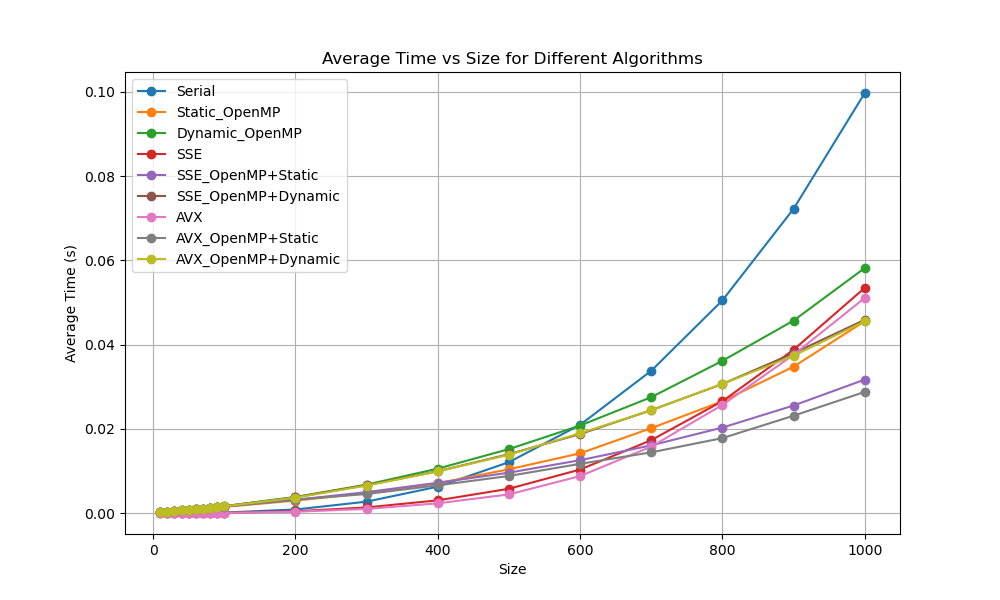
\includegraphics[width=0.45\textwidth]{fig/fig5.png}
    }
    \subfigure[运行时间对数尺度下性能比较]{
        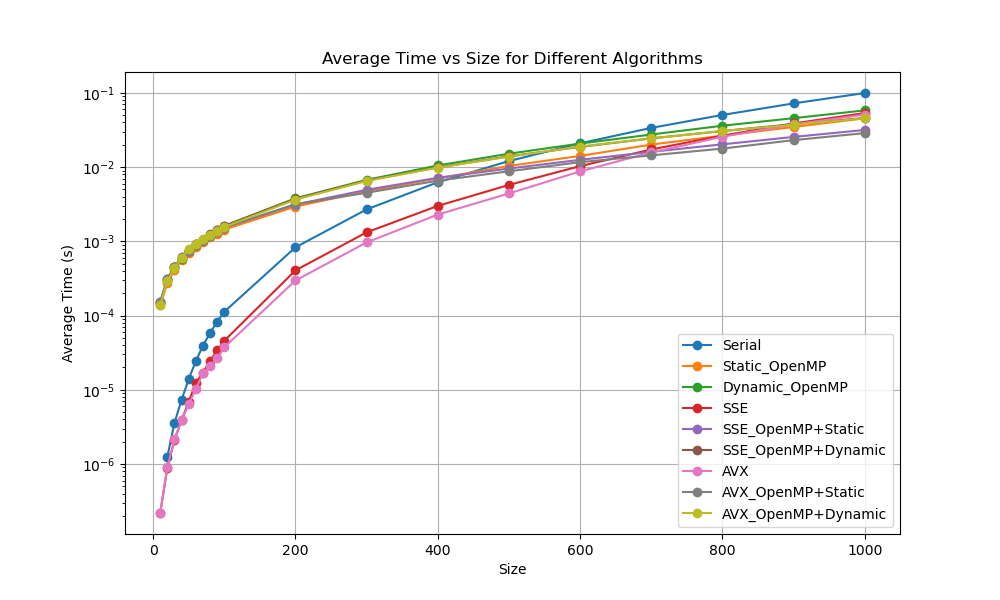
\includegraphics[width=0.45\textwidth]{fig/fig6.png}
    }
    \caption{多尺度性能比较}
\end{figure}

上述两张图片分别从线性尺度和对数尺度两个不同度量标准(对运行时间)上展示了各种算法
运行时间随着规模增大的变化情况。其中,线性尺度适合观察大矩阵时的性能差异,对数尺度有助于展示小矩阵时的性能差异。

观察上述图片,可以得到以下结论:
\begin{enumerate}
    \item 当测试矩阵规模较小时,各单线程串行版本高斯消元明显优于其所对应的基于OpenMP的多线程版本高斯消元
    \item 当测试矩阵规模较大时,各基于OpenMP的多线程版本高斯消元明显优于其所对应的单线程串行版本高斯消元
    \item 在单线程版本高斯消元中,总的来看,使用AVX性能最优,SSE次之且与AVX性能接近,普通串行版本性能最差
    \item 在基于OpenMP的多线程静态任务分配版本高斯消元中,总的来看,AVX性能最优,SSE性能次之且与AVX性能接近,为优化多线程静态任务分配性能最差
    \item 在基于OpenMP的多线程动态任务分配版本高斯消元中,总的来看,AVX与SSE性能接近且明显优于未优化多线程动态分配版本的高斯消元
    \item 在未使用向量编程的高斯消元中,总的来看,性能比较为:\textbf{静态任务分配 > 动态任务分配 > 普通串行版本}
    \item 在使用SSE向量编程的高斯消元中,总的来看,性能比较为:\textbf{静态任务分配 > 动态任务分配 > SSE单线程版本}
    \item 在使用AVX向量编程的高斯消元中,总的来看,性能比较为:\textbf{静态任务分配 > 动态任务分配 > AVX单线程版本}
\end{enumerate}

综合上述考量,以下是对上述实验结果的分析:
\begin{enumerate}
    \item \textbf{小规模矩阵下,单线程优于多线程}
    \begin{itemize}
        \item 小规模矩阵的计算量较低,单线程串行执行无需额外的线程创建、同步、通信等开销,因此性能更优。
        \item 多线程在这种场景下会因线程管理和任务分配的开销导致性能下降,甚至可能超过计算本身的开销。
    \end{itemize}

    \item \textbf{大规模矩阵下,多线程优于单线程}
    \begin{itemize}
        \item 随着矩阵规模增大,计算复杂度呈指数级上升,多线程可以有效利用多核资源分担计算任务。
        \item 大规模矩阵的计算时间远大于多线程的管理开销,因此总体性能提升显著。
    \end{itemize}

    \item \textbf{单线程版本中,总的来看,AVX > SSE > 普通串行}
    \begin{itemize}
        \item AVX和SSE是矢量化指令集,能够一次处理多个浮点数运算,显著提升并行计算能力。
        \item AVX的寄存器宽度为256位,比SSE的128位更宽,能够一次处理更多数据,因此性能更优。
        \item 普通串行版本每次仅处理一个元素,计算效率最低。
    \end{itemize}

    \item \textbf{多线程静态任务分配中,总的来看,AVX >(略大于) SSE > 普通串行}
    \begin{itemize}
        \item 静态任务分配在计算密集型任务中表现更优,因为任务分配的开销只发生一次,之后线程间几乎无通信。
        \item AVX优化进一步加速了每个线程的计算过程,结合静态任务分配的低开销,使性能达到最佳。
    \end{itemize}

    \item \textbf{多线程动态任务分配中,总的来看,AVX >(略大于) SSE > 普通串行}
    \begin{itemize}
        \item 动态任务分配灵活性更强,但任务调度和线程间同步的开销较高。
        \item AVX和SSE的性能差异在动态任务分配的调度开销下被部分掩盖,因此两者表现相近。
    \end{itemize}

    \item \textbf{未使用向量优化版本中,总的来看,静态任务分配优于动态任务分配,且都优于单线程}
    \begin{itemize}
        \item 静态任务分配在任务分布均匀的情况下,避免了动态调度的额外开销,因此性能更优。在本人任务中,任务负载较为均衡,故静态任务调度优于动态任务调度。
        \item 动态分配虽然具有灵活性,但在任务负载平衡较好的情况下,这种灵活性带来的开销反而显得多余。(本次任务中就有所体现)
        \item 而多线程通过并行处理任务充分利用多核资源、隐藏延迟、提升响应速度,从而在计算密集或任务负载较大的场景中显著优于单线程。
    \end{itemize}

    \item \textbf{使用SSE或AVX时,总的来看,静态任务分配仍优于动态分配,且都优于单线程}
    \begin{itemize}
        \item SSE和AVX优化提升了线程的计算效率,而静态任务分配的低管理开销放大了这种优势。
        \item 动态分配开销较高,即使结合矢量化优化,也无法完全弥补调度上的劣势。
        \item 而多线程通过并行处理任务充分利用多核资源、隐藏延迟、提升响应速度,从而在计算密集或任务负载较大的场景中显著优于单线程。
    \end{itemize}

    \item \textbf{相同任务分配策略下,总的来看,AVX > SSE > 无向量优化}
    \begin{itemize}
        \item AVX和SSE通过硬件加速实现数据级并行,性能优于传统计算方式。
        \item AVX的寄存器更宽,执行效率更高,使其性能略优于SSE。
    \end{itemize}
\end{enumerate}

\subsection{思考总结}
通过本次实验,我们进一步理解了计算资源利用与优化策略选择的内在逻辑,即:
\begin{itemize}
    \item \textbf{当我们面临小规模任务时:}避免多线程开销,直接采用高效单线程优化(如AVX)
    \item \textbf{当我们面临大规模任务时:}充分利用多线程结合矢量化优化,静态任务分配在负载均衡时是首选,动态分配适合不确定性任务。
    \item \textbf{硬件指令集优化:}在支持的硬件平台上,优先考虑AVX以充分发挥现代处理器的并行计算能力。
\end{itemize}

另外,我深刻体会到了并行计算的强大力量。利用OpenMP进行多线程处理,显著提升了大规模矩阵运算的效率,这让我更加理解了在合适的场景下,合理利用多核资源的重要性。
同时,SSE和AVX指令集的应用让我意识到硬件优化的潜力。它们通过矢量化计算大幅提高了单线程的性能,尤其是在小规模任务中,避免了多线程带来的额外开销。
这次实验让我更加明确了在不同任务规模下选择合适优化策略的必要性,并对现代计算机体系结构有了更深入的理解。

希望能在下节实验课学到更多有用并且有趣的知识:)
\end{document}